%% Run LaTeX on this file several times to get Table of Contents,
%% cross-references, and citations.

\documentclass[11pt]{book}
\usepackage{gvv}
\usepackage{gvv-book-bkup}
%\usepackage{Wiley-AuthoringTemplate}
\usepackage[sectionbib,authoryear]{natbib}% for name-date citation comment the below line
%\usepackage[sectionbib,numbers]{natbib}% for numbered citation comment the above line

%%********************************************************************%%
%%       How many levels of section head would you like numbered?     %%
%% 0= no section numbers, 1= section, 2= subsection, 3= subsubsection %%
\setcounter{secnumdepth}{3}
%%********************************************************************%%
%%**********************************************************************%%
%%     How many levels of section head would you like to appear in the  %%
%%				Table of Contents?			%%
%% 0= chapter, 1= section, 2= subsection, 3= subsubsection titles.	%%
\setcounter{tocdepth}{2}
%%**********************************************************************%%
\setcounter{tocdepth}{3}
%\includeonly{ch01}
\makeindex

\begin{document}

\frontmatter
%%%%%%%%%%%%%%%%%%%%%%%%%%%%%%%%%%%%%%%%%%%%%%%%%%%%%%%%%%%%%%%%
%% Title Pages
%% Wiley will provide title and copyright page, but you can make
%% your own titlepages if you'd like anyway
%% Setting up title pages, type in the appropriate names here:

\booktitle{CBSE Math}

\subtitle{Made Simple}

\AuAff{G. V. V. Sharma}


%% \\ will start a new line.
%% You may add \affil{} for affiliation, ie,
%\authors{Robert M. Groves\\
%\affil{Universitat de les Illes Balears}
%Floyd J. Fowler, Jr.\\
%\affil{University of New Mexico}
%}

%% Print Half Title and Title Page:
%\halftitlepage
\titlepage

%%%%%%%%%%%%%%%%%%%%%%%%%%%%%%%%%%%%%%%%%%%%%%%%%%%%%%%%%%%%%%%%
%% Copyright Page

\begin{copyrightpage}{2023}
%Title, etc
\end{copyrightpage}

% Note, you must use \ to start indented lines, ie,
% 
% \begin{copyrightpage}{2004}
% Survey Methodology / Robert M. Groves . . . [et al.].
% \       p. cm.---(Wiley series in survey methodology)
% \    ``Wiley-Interscience."
% \    Includes bibliographical references and index.
% \    ISBN 0-471-48348-6 (pbk.)
% \    1. Surveys---Methodology.  2. Social 
% \  sciences---Research---Statistical methods.  I. Groves, Robert M.  II. %
% Series.\\

% HA31.2.S873 2004
% 001.4'33---dc22                                             2004044064
% \end{copyrightpage}

%%%%%%%%%%%%%%%%%%%%%%%%%%%%%%%%%%%%%%%%%%%%%%%%%%%%%%%%%%%%%%%%
%% Only Dedication (optional) 

%\dedication{To my parents}

\tableofcontents

%\listoffigures %optional
%\listoftables  %optional

%% or Contributor Page for edited books
%% before \tableofcontents

%%%%%%%%%%%%%%%%%%%%%%%%%%%%%%%%%%%%%%%%%%%%%%%%%%%%%%%%%%%%%%%%
%  Contributors Page for Edited Book
%%%%%%%%%%%%%%%%%%%%%%%%%%%%%%%%%%%%%%%%%%%%%%%%%%%%%%%%%%%%%%%%

% If your book has chapters written by different authors,
% you'll need a Contributors page.

% Use \begin{contributors}...\end{contributors} and
% then enter each author with the \name{} command, followed
% by the affiliation information.

% \begin{contributors}
% \name{Masayki Abe,} Fujitsu Laboratories Ltd., Fujitsu Limited, Atsugi, Japan
%
% \name{L. A. Akers,} Center for Solid State Electronics Research, Arizona State University, Tempe, Arizona
%
% \name{G. H. Bernstein,} Department of Electrical and Computer Engineering, University of Notre Dame, Notre Dame, South Bend, Indiana; formerly of
% Center for Solid State Electronics Research, Arizona
% State University, Tempe, Arizona 
% \end{contributors}

%%%%%%%%%%%%%%%%%%%%%%%%%%%%%%%%%%%%%%%%%%%%%%%%%%%%%%%%%%%%%%%%
% Optional Foreword:

%\begin{foreword}
%\lipsum[1-2]
%\end{foreword}

%%%%%%%%%%%%%%%%%%%%%%%%%%%%%%%%%%%%%%%%%%%%%%%%%%%%%%%%%%%%%%%%
% Optional Preface:

%\begin{preface}
%\lipsum[1-1]
%\prefaceauthor{}
%\where{place\\
% date}
%\end{preface}

% ie,
% \begin{preface}
% This is an example preface.
% \prefaceauthor{R. K. Watts}
% \where{Durham, North Carolina\\
% September, 2004}

%%%%%%%%%%%%%%%%%%%%%%%%%%%%%%%%%%%%%%%%%%%%%%%%%%%%%%%%%%%%%%%%
% Optional Acknowledgments:

%\acknowledgments
%\lipsum[1-2]
%\authorinitials{I. R. S.}  

%%%%%%%%%%%%%%%%%%%%%%%%%%%%%%%%
%% Glossary Type of Environment:

% \begin{glossary}
% \term{<term>}{<description>}
% \end{glossary}

%%%%%%%%%%%%%%%%%%%%%%%%%%%%%%%%
%\begin{acronyms}
%\acro{ASTA}{Arrivals See Time Averages}
%\acro{BHCA}{Busy Hour Call Attempts}
%\acro{BR}{Bandwidth Reservation}
%\acro{b.u.}{bandwidth unit(s)}
%\acro{CAC}{Call / Connection Admission Control}
%\acro{CBP}{Call Blocking Probability(-ies)}
%\acro{CCS}{Centum Call Seconds}
%\acro{CDTM}{Connection Dependent Threshold Model}
%\acro{CS}{Complete Sharing}
%\acro{DiffServ}{Differentiated Services}
%\acro{EMLM}{Erlang Multirate Loss Model}
%\acro{erl}{The Erlang unit of traffic-load}
%\acro{FIFO}{First in - First out}
%\acro{GB}{Global balance}
%\acro{GoS}{Grade of Service}
%\acro{ICT}{Information and Communication Technology}
%\acro{IntServ}{Integrated Services}
%\acro{IP}{Internet Protocol}
%\acro{ITU-T}{International Telecommunication Unit -- Standardization sector}
%\acro{LB}{Local balance}
%\acro{LHS}{Left hand side}
%\acro{LIFO}{Last in - First out}
%\acro{MMPP}{Markov Modulated Poisson Process}
%\acro{MPLS}{Multiple Protocol Labeling Switching}
%\acro{MRM}{Multi-Retry Model}
%\acro{MTM}{Multi-Threshold Model}
%\acro{PASTA}{Poisson Arrivals See Time Averages}
%\acro{PDF}{Probability Distribution Function}
%\acro{pdf}{probability density function}
%\acro{PFS}{Product Form Solution}
%\acro{QoS}{Quality of Service}
%\acro{r.v.}{random variable(s)}
%\acro{RED}{random early detection}
%\acro{RHS}{Right hand side}
%\acro{RLA}{Reduced Load Approximation}
%\acro{SIRO}{service in random order}
%\acro{SRM}{Single-Retry Model}
%\acro{STM}{Single-Threshold Model}
%\acro{TCP}{Transport Control Protocol}
%\acro{TH}{Threshold(s)}
%\acro{UDP}{User Datagram Protocol}
%\end{acronyms}

\setcounter{page}{1}

\begin{introduction}
This book links high school coordinate geometry to linear algebra and matrix analysis through solved problems.

\end{introduction}

\mainmatter
\chapter{Vectors}
\section{2023}
\subsection{10}
\input{2023/vectors10-1.tex}
\subsection{10}

\begin{enumerate}

\item Find a unit vector perpendicular to both the vectors $\overrightarrow{a} $ and $\overrightarrow{b} ,$ where 
       $\overrightarrow{a} $ =$\hat{i} -7 \hat{j} + 7\hat{k}$ and
       $\overrightarrow{b} $ =$3\hat{i} -2 \hat{j} + 2\hat{k}.$
       

    \item Show that the vectors $\hat{i} -2 \hat{j} + 3\hat{k}$ and $\hat{i} -3 \hat{j} + 5\hat{k}$
are coplanar.
    \item Let $\overrightarrow{a} $,\hspace{5pt} $\overrightarrow{b} $, and \hspace{5pt}$\overrightarrow{c} $ be three vectors such that $|\overrightarrow{a}|$=1,\hspace{5pt}$|\overrightarrow{b}|$=2 and \hspace{5pt}$|\overrightarrow{c}|$=3.If the projection of \hspace{5pt}$\overrightarrow{b} $ along \hspace{5pt}$\overrightarrow{a}$ is equal to the projection of \hspace{5pt}$\overrightarrow{c} $ along \hspace{5pt}$\overrightarrow{a}$ ; and  \hspace{5pt}$\overrightarrow{b} $ , \hspace{5pt}$\overrightarrow{c} $ are perpendicular to each other, then find $|3 \overrightarrow{a}- 2 \overrightarrow{b} + 2\overrightarrow{c} |$.
    \item Find the vector and cartesian equations of the plane passing through the points \brak{2, 5, - 3}, \brak{-2, -3, 5}  and \brak{5, 3, - 3}. Also, find the point of intersection of this plane with the line passing through points \brak{3, 1, 5} and \brak{-1, -3, -1}.

    \item Find the equation of the plane passing through the intersection of the planes $\overrightarrow{r}$ .\hspace{1.5pt} $\brak{\hat{i} + \hat{j} + \hat{k}} =1 $ and $\overrightarrow{r}$ .\hspace{1.5pt} $\brak{2\hat{i} + 3\hat{j} - \hat{k}}$ + 4 = 0 and parallel to x-axis. Hence, find the distance of the plane from x-axis.

 \end{enumerate}

\subsection{12}
\input{2023/vector12-1.tex}
\section{2022}
\subsection{10}
\input{2022/maths1.tex}
\subsection{12}
\begin{enumerate}
\item Find the coordinates of a point $\vec{A}$, where $\vec{AB}$ is diameter of a circle whose center is $\brak{2,-3}$ and $\vec{B}$ is the point $\brak{1,4}$.
\item Find the ratio in which the segment joining the points $\brak{1, 3}$ and $\brak{4, 5}$ is divided by $x-axis$? Also find the coordinates of this point on  $x$-axis.
\item Find the point on $y-axis$ which is equidistant from the points $\brak{5, -2}$ and $\brak{-3, 2}$.    
\item The line segment joining the points $\vec{A}\brak{2, 1}$ and $\vec{B}\brak{5, -8}$ is trisected at the points $\vec{P}$ and $\vec{Q}$ such that $\vec{P}$ is nearer to $\vec{A}$. If $\vec{P}$ also lies on the line given by $2x-y+k=0$, find the value of $k$.
\item Find the coordinates of a point $A$, where $AB$ is a diameter of the circle with centre $(-2, 2)$ and $B$ is the point with coordinates $(3, 4)$.
\end{enumerate}
\section{2021}
\subsection{10}
\input{2021/Vectors-10}
\subsection{12}
\input{2021/vectors21-12.tex}
\chapter{Linear Forms}
\section{2023}
\subsection{10}
\input{2023/linear-10th.tex}
\subsection{12}                                                                                                  
\documentclass[12pt,A4 paper]{article}
\usepackage{mathtools}
\usepackage{graphicx}
\usepackage{gensymb}
\begin{document}
\title{\textbf{LINEAR}}
\date{}
\maketitle
\begin{enumerate}
    \item Equation of line passing through origin and making $30\degree,60\degree$ and $90\degree$ with $x,y,z$ axes respectively is
    \begin{enumerate}
        \item $\frac{2x}{\sqrt3}=\frac{y}{2}=\frac{z}{0}$
        \item $\frac{2x}{\sqrt3}=\frac{2y}{1}=\frac{z}{0}$
        \item $2x=\frac{2y}{\sqrt3}=\frac{z}{1}$
        \item $\frac{2x}{\sqrt3}=\frac{2y}{1}=\frac{z}{1}$
    \end{enumerate}
    \item If the equation of a line is $x=ay+b,z=cy+d$,then find the direction ratios of the line and a point on the line.
    \item
    \begin{enumerate}
        \item Find the equations of the diagonals of the parallelogram $PQRS$ whose vertices are$P(4,2,-6),Q(5,-3,1),R(12,4,5),S(11,9,-2)$.Use these equations to find the point of intersection of diagonals.  
        \item A line $l$ passes through point$(-1,3,-2)$ and is perpendicular to both the lines $\frac{x}{1}=\frac{y}{2}=\frac{z}{3}$ and $\frac{x+2}{-3}=\frac{y-1}{2}=\frac{z+1}{5}$.Find the vector equation of the line $l$.Hence,obtain its distance from origin.
    \end{enumerate}
   
   
   
\end{enumerate}
\end{document}


\section{2022}
\begin{enumerate}[label=\thesection.\arabic*.,ref=\thesection.\theenumi]
\numberwithin{equation}{enumi}
\numberwithin{figure}{enumi}
\numberwithin{table}{enumi}

	\item Solve the equations $x+2y=6$ and $2x-5y=12$ graphically.	

	\item Solve the following equations for $x$ and $y$ using cross-multiplication method:
		\begin{align}
			(ax-by)+(a+4b)=0\\(bx+ay)+(b-4a)=0
		\end{align}

	\item Find the co-ordinates of the point where the line $\dfrac{x-3}{-1}=\dfrac{y+4}{1}=\dfrac{z+5}{6}$ crosses the plane passing through the points $\left(\dfrac{7}{2},0,0\right),(0,7,0),(0,0,7)$.

	\item Electrical transmission wires which are laid down in winters are stretched tightly to accommodate expansion in summers.
		\begin{figure}[H]
			\centering
			\includegraphics[width=\columnwidth]{figs/txn}
			\caption{Electrical transmission wires connected to a transmission tower.}
			\label{fig:txn1}
		\end{figure}
		Two such wires in the figure \ref{fig:txn1} lie along the following lines:
		\begin{align}
			l_1 &: \dfrac{x+1}{3}=\dfrac{y-3}{-2}=\dfrac{z+2}{-1}\\
			l_2 &: \dfrac{x}{-1}=\dfrac{y-7}{3}=\dfrac{z+7}{-2}
		\end{align}
		Based on the given information, answer the following questions:
		\begin{enumerate}
			\item	Are the $l_1$ and $l_2$ coplanar? Justify your answer.
			\item    Find the point of intersection of lines $l_1$ and $l_2$.
		\end{enumerate}

	\item Write the cartesian equation of the line PQ passing through points P$(2,2,1)$ and Q$(5,1,-2)$. Hence, find the y-coordinate of the point on the line PQ whose z-coordinate is -2.

	\item Find the distance between the lines $x=\dfrac{y-1}{2}=\dfrac{z-2}{3}$ and $x+1=\dfrac{y+2}{2}=\dfrac{z-1}{3}$.
	
	\item Find the shortest distance between the following lines:
		\begin{align}
			\vec{r}&=3\hat{i}+5\hat{j}+7\hat{k}+\lambda(\hat{i}-2\hat{j}+\hat{k})\\\vec{r}&=(-\hat{i}-\hat{j}-\hat{k})+\mu(7\hat{i}-6\hat{j}+\hat{k})
		\end{align}

	\item Two motorcycles A and B are running at a speed more than the allowed speed on the road (as shown in figure \ref{fig:bike1}) represented by the following lines 
		\begin{align}
			\vec{r}&=\lambda(\hat{i}+2\hat{j}-\hat{k})\\\vec{r}&=(3\hat{i}+3\hat{j})+\mu(2\hat{i}+\hat{j}+\hat{k})
		\end{align}
		\begin{figure}[H]
			\centering
			\includegraphics[width=\columnwidth]{figs/bike}
			\caption{Two motorcycles moving along the road in a straight line.}
			\label{fig:bike1}
		\end{figure}
		Based on the following information, answer the following questions:
		\begin{enumerate}
			\item Find the shortest distance between the given lines.
			\item Find a point at which the motorcycles may collide.
		\end{enumerate}
	
	\item Find the shortest distance between the following lines
		\begin{align}
			\vec{r}&=(\lambda+1)\hat{i}+(\lambda+4)\hat{j}-(\lambda-3)\hat{k}\\\vec{r}&=(3-\mu)\hat{i}+(2\mu+2)\hat{j}+(\mu+6)\hat{k}
		\end{align}
	
	\item Find the shortest distance between the following lines and hence write whether the lines are intersecting or not.
		\begin{align}
			\dfrac{x-1}{2}=\dfrac{y+1}{3}=z, \dfrac{x+1}{5}=\dfrac{y-2}{1}, z=2
		\end{align}
\item Find the equation of the plane passing through the points $(2,1,0),(3,-2,-2)$ and $(1,1,7)$. Also, obtain its distance from the origin.

	\item The foot of a perpendicular drawn from the point $(-2,-1,-3)$ on a plane is $(1,-3,3)$. Find the equation of the plane.

	\item Find the cartesian and the vector equation of a plane which passes through the point $(3,2,0)$ and contains the line $\dfrac{x-3}{1}=\dfrac{y-6}{5}=\dfrac{z-4}{4}$.

	\item The distance between the planes $4x-4y+2z+5=0$ and $2x-2y+z+6=0$ is

		\begin{enumerate}

			\item $\dfrac{1}{6}$
			\item $\dfrac{7}{6}$
			\item $\dfrac{11}{6}$
			\item $\dfrac{16}{6}$
		\end{enumerate}

	\item Find the equation of the plane through the line of intersection of the planes
		\begin{align}
			\vec{r}\cdot(\hat{i}+3\hat{j})+6&=0\\\vec{r}\cdot(3\hat{i}-\hat{j}-4\hat{k})&=0
		\end{align}which is at a  unit distance from the origin.

		\item If the distance of the point $(1,1,1)$ from the plane $x-y+z+\lambda=0$ is $\dfrac{5}{\sqrt{3}}$, find the value(s) of $\lambda$.

	\item Find the distance of the point $(2,3,4)$ measured along the line $\dfrac{x-4}{3}=\dfrac{y+5}{6}=\dfrac{z+1}{2}$ from the plane $3x+2y+2z+5=0$.

	\item Find the distance of the point $P(4,3,2)$ from the plane determined by the points $A(-1,6,-5),B(-5,-2,3)$ and $C(2,4,-5)$.

	\item The distance of the line
		\begin{align}
		\vec{r}=(\hat{i}-\hat{j})+\lambda(\hat{i}+5\hat{j}+\hat{k})\end{align}
		from the plane
		\begin{align}
		\vec{r}\cdot(\hat{i}-\hat{j}+4\hat{k})=5\end{align}
		is
		\begin{enumerate}
			\item $\sqrt{2}$
			\item $\dfrac{1}{\sqrt{2}}$
			\item $\dfrac{1}{3\sqrt{2}}$
			\item $\dfrac{-2}{3\sqrt{2}}$
		\end{enumerate}

	\item Find a unit vector perpendicular to each of the vectors $(\vec{a}+\vec{b})$ and $(\vec{a}-\vec{b})$ where 
	\begin{align}
		\vec{a}&=\hat{i}+\hat{j}+\hat{k}\\\vec{b}&=\hat{i}+2\hat{j}+3\hat{k}
	\end{align}

\item Find the distance of the point $(1,-2,9)$ from the point of intersection of the line
		\begin{align}
			\vec{r}=4\hat{i}+2\hat{j}+7\hat{k}+\lambda(3\hat{i}+4\hat{j}+2\hat{k})
		\end{align}and the plane
		\begin{align}
			\vec{r}\cdot(\hat{i}-\hat{j}+\hat{k})=10.
		\end{align}

	\item Find the area bounded by the curves $y=\abs{x-1}$ and $y=1$, using integration.

	\item Find the coordinates of the point where the line through $(4,-3,-4)$ and $(3,-2,2)$ crosses the plane $2x+y+z=6$.

	\item Fit a straight line trend by the method of least squares and find the trend value for the year 2008 using the data from Table \ref{tab:LC}:
		\begin{table}[H]
			\caption{Table showing yearly trend of production of goods in lakh tonnes \label{tab:LC}}
			\input{2022/table2}
		\end{table}
		\end{enumerate}

\section{2021}
\subsection{10}
\input{2021/linearforms.tex}
\subsection{12}
\begin{enumerate}
    \item If the two lines
    \begin{align}
          L_1 : x=5,\frac{y}{3-\alpha}=\frac{z}{-2}\\
         L_1 : x=2,\frac{y}{-1}=\frac{z}{z-\alpha} 
       \end{align}
  are perpendicular,then the value of $\alpha$ 
        \begin{enumerate}
        \item $\frac{2}{3}$
        \item $3$
        \item $4$
        \item $\frac{7}{3}$
    \end{enumerate}

    \item Find the shortest distance between the following lines and hence write
whether the lines are intersecting or not.
\begin{align}
    \frac{x-1}{2} &= \frac{y+1}{3} = z \\
    \frac{x+1}{5} &=\frac{y-2}{1},z=2
\end{align}

\item  Find the equation of the plane through the line of intersection of the planes 
\begin{align}
     \vec{r} .\brak{i+3j} + 6 &= 0 \\  \vec{r} .\brak{3i - j - 4k} &= 0
\end{align}
which is at a unit distance from the origin.
    \item If segment of the line intercepted between the co-ordinate-axes is bisected
at the point $M\brak{2, 3}$, then the equation of this line is
 \begin{align}
       2x + 3y &= 13\\
       x + y &= 5 \\
       2x + y &= 7\\
       3x + 2y &= 12
\end{align}
\item The equation of a line through $(2,-4)$ and parallel to x-axis is $\underline{\hspace{2cm}}$.
\item Find the equation of the median through vertex $A$ of the triangle $ABC$, having vertices $A\brak{2,5}$, $B\brak{-4,9}$ and $C\brak{-2, -1}$.
\item Solve the system of linear equations, using matrix method : 
\begin{align}
  7x + 2y &= 11\\
 4x - y &= 2
\end{align}
\end{enumerate}

\chapter{Circles}

\begin{enumerate}[label=\thesection.\arabic*.,ref=\theenumi]
		\numberwithin{equation}{enumi}
	\item In tangents $\vec{PA}$ and $\vec{PB}$ from an external point $P$ to a circle with centre $O$ , are inclined to each other at an angle of $80^{\degree}$, then $\angle AOB$ is equal to
 \begin{figure}[H]
        \centering
        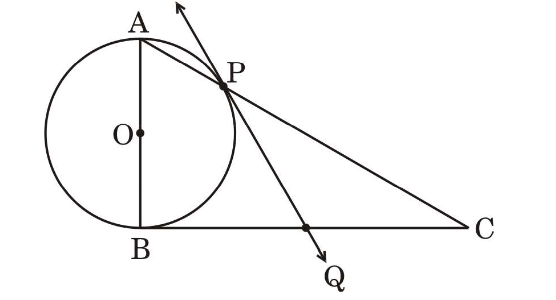
\includegraphics[width = \columnwidth]{figs/Tan_circle23.png}
        \caption{Tangents $PA$ and $PB$}
        \label{fig:Tan_circle23}
    \end{figure}
    \begin{enumerate}
        \item $100^{\degree}$
        \item $60^{\degree}$
        \item $100^{\degree}$
        \item $100^{\degree}$
    \end{enumerate}

    \item  Two concentric circles are of radii $4 cm$ and $3 cm$. Find the length of the chord of the larger circle which touches the smaller circle.

    \item  In a triangle $ABC$ with $\angle AOB$ is shown. Taking $AB$ as diameter, a circle has been drawn intersecting $AC$ at point $P$. Prove that the tangent drawn at point $P$ bisects $BC$. 
	    \begin{figure}[H]
            \centering
                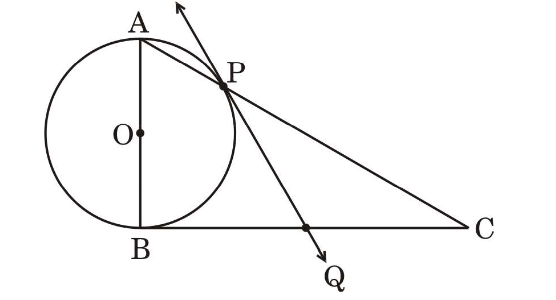
\includegraphics[width = \columnwidth]{figs/concen_circle23.png}
                \caption{Concentric circles}
                \label{fig:concen_circle23}
        \end{figure}
    \item  Prove that a Parallelogram circumscribing a circle is a rhombus.
     \item  In two circles with centres at $O$ and $O$ of radii $2r$ and $r$ respectively, touch each other internally at $A$. A chord $AB$ of the bigger circle meets the smaller circle at $C$. Show that  $C$ bisects $AB$.
    \begin{figure}[H]
        \centering
        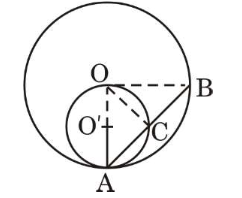
\includegraphics[width = \columnwidth]{figs/two_circle23.png}
        \caption{Two circles with center}
        \label{fig:two_circle23}
    \end{figure}  
    
    \item In $O$ is centre of a circle of radius $5 cm$. $PA$ and $BC$ are tangents to the circle at $A$ and $B$ respectively. If $OP = 13 cm$, then find the length of tangents $PA$ and $BC$.
\begin{figure}[H]                                                                                             
\centering                                                                                                
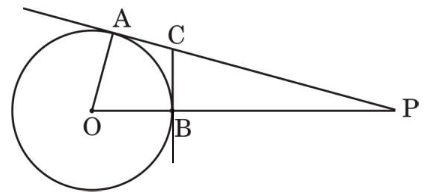
\includegraphics[width = \columnwidth]{figs/circle_radius23.png}
\caption{The center of circle radius is $5cm$}
\label{fig:circle_radius23}        
\end{figure}

    \item In two concentric circles, a chord of length $48 cm$ of the larger
circle is a tangent to the smaller circle, whose radius is $7 cm$. Find the radius of the larger circle. 
    \item At a point on the level ground, the angle of elevation of the top
of a vertical tower is found to be $\alpha$, such that $\tan \alpha =\frac{5}{12} $. On walking $192 m$ towards the tower, the angle of elevation $\beta$ is such that $\tan \beta=\frac{3}{4}$. Find the height of the tower. 
\end{enumerate}

\section{2022}
\subsection{10}
\section{2023}
\subsection{10}
\input{2023/Circle10.tex}
\section{2022}
\input{2022/tangent1.tex}
\section{2021}
\subsection{10}
\input{2021/circle-10.tex}
\chapter{Intersection of Conics}
\section{2022}
\input{2022/chords.tex}
\section{2021}
\subsection{12}
\begin{enumerate}
        \item The point at which the normal to the curve 
\begin{align}
    y = x+\frac{1}{x}, x>0 
\end{align}
 is perpendicular to the line
 \begin{align}
     3x-4y-7 = 0 
 \end{align}
\begin{enumerate}
    \item $\brak{2,\frac{5}{2}}$   \item $\brak{\pm2,\frac{5}{2}}$  

         \item $\brak{-\frac{1}{2},\frac{5}{2}}$    \item $\brak{\frac{1}{2},\frac{5}{2}}$
\end{enumerate}
         
         \item The points on the curve
         \begin{align}
             \frac{x^2}{9} +\frac{y^2}{16} = 1
         \end{align}
         at which the tangents are parallel to $y$-axis are:
         \begin{enumerate}
             \item $\brak{0,\pm4}$   \item $\brak{\pm4,0}$  

         \item  $\brak{\pm3,0}$   \item $\brak{0,\pm3}$
         \end{enumerate}
           
         \item For which value of m is the line
         \begin{align}
            y = mx + 1 
         \end{align}a tangent to the curve 
        \begin{align}
            y^2 = 4x 
        \end{align}
        \begin{enumerate}
            \item  $\frac{1}{2}$  \item $1$

         \item 2  \item 3
        \end{enumerate}
\end{enumerate}

\chapter{Probability}
\section{2021}
\subsection{10}
\begin{enumerate}
\item Let A and B be two events such that $P(A) = \frac{5}{8}$, $P(B) = \frac{1}{2}$ and  $P(A|B) = \frac{3}{4}$. Find the value of $P(B|A)$.
\item Two balls are drawn at random from a bag containing 2 red balls and 3 blue balls, without replacement. Let the variables X denotes the number of red balls. Find the probabillity distribution of X.
\item A card from a pack of 52 playing cards is lost. From the remaining cards, 2 cards are drawn at random without replacement, and are found to be both aces. Find the probability that lost card being an ace.
\item Probabilities of A and B solving a specific problem are $\frac{2}{3}$ and $\frac{3}{5},$ respectively. If both of them try independently to solve the problem, then find the probability that the problem is  solved.
\item A pair of dice is thrown. It is given that the sum of numbers  appearing on both dice is an even number. Find the probability that the number apprearing on at least one die is 3.
\item At the start of a cricket match, a coin is tossed and the team winning the toss has the opportunity to choose to bat or bowl. such a coin is unbaised with equal probabilities of getting head and tail\figref{fig:coin1} .
\begin{figure}[!ht]
\centering
\includegraphics[width=\columnwidth]{figs/coin}
\caption{Toss before the match}
\label{fig:coin1}
\end{figure}
\\ Based on the above information, answer the following question:
\begin{enumerate}
\item If such a coin is tossed 2 times, then find the probability distibution of numbers of tails.
\item Find the probability of getting at least one head in three tosses of such a coin.
\end{enumerate}
\item Two cards are drawn successively with replacement from a well shuffled pack of 52 cards. Find the probability distribution of the number of spade cards.
\item A pair of dice is thrown and the sum of the numbers appearing on the dice is observed to be 7. Find the probability that the number 5 has appeared on at least one die.
\item The probability that A hits the target is $\frac{1}{3}$ and the probability that B hits it, is $\frac{2}{5}.$ If both try to hit the target independently, find the probabillity that the target is hit. 
\item A shopkeeper sells three types of flower seeds A$_1$ , A$_1$ , A$_3$. They are sold in the form of a mixture, where the proportions of these seeds are  4 : 4 : 2, respectively. The germinaton rates of the three types of seeds are $45\%,$ $60\%$ and $35\%$ respectively\figref{fig:flowers11}.
\begin{figure}[!ht]
\centering                                  \includegraphics[width=\columnwidth]{figs/flowers}                                     
\caption{Three types of flowers}            
\label{fig:flowers11}                       
\end{figure}
\\ Based on  the above information :
\begin{enumerate}
\item  Calculate the probability that a randomly chosen seed will germinate.
\item  Calculate the probability  that the seed is of type $A_2$, given that a randomly choosen seed germinates.
\end{enumerate}
\item Three friends A, B and C got their photograph clicked. Find the probability that B is standing at the central position, given that A is standing at the left corner.
\item In a game of Archery, each ring of the Archery target is valued. The centremost ring is worth 10 points and rest of the rings are alloted points 9 to 1 in sequential order moving outwards.Archer A is likely to earn 10 points with a probability of 0.8 and Archer B is likely the earn 10 points with a probability of 0.9\figref{fig:archery3}.
\begin{figure}[!ht]                     
\centering
\includegraphics[width=\columnwidth]{figs/archery}
\caption{centermost ring}                   
\label{fig:archery3}                        
\end{figure}
\\ Based on the above innformation, answer the following questions :
\begin{enumerate}
\item exactly one of them earns 10 points .
\item both of them earn 10 point.
\end{enumerate}
\item Event A and B are such that \begin{align} P(A) = \frac{1}{2},  P(B) = \frac{7}{12}\end{align} and \begin{align} P(\bar{A}\cup \bar{B}) = \frac{1}{4} \end{align}
Find whether the events  A and B are independent or not.
\item A box $B_1$ contain 1 white ball  and 3 red balls. Another box $B_2$ contains 2 white balls and 3 red balls. If one ball is drawn at random from each of the boxes $B_1$ and $B_2$, then find the probability that the two balls drawn are of the same colour.
\item Let X be random variable which assumes values $x_1$, $x_2$, $x_3$, $x_4$  such that\begin{align} 2P(X = x_1) = 3P (X = x_2) = P ( X = x_3) = 5P (X = x_4).\end{align}
\\ Find the probability distribution of X.
\item There are two boxes, namely box-I and box-II. Box-I contains  3 red and 6 black balls. Box-II contains 5 red and 5 black balls. One of the two boxes , is selected at random and a ball is drawn at random. The ball drawn is found to be red. Find the probability that this red ball comes out from box-II.
\item In a toss of three different coins, find the probability of comming up of three heads, if it is known that at least one head comes up.
\item A laboratory blood text is $98\%$ effective  in detecting a certain disease when it is fact, present. However, the text also yeilds a false positive result for $0.4\%$ of the healthy person tested. From a large population, it is given that $0.2\%$ of the population actually has the diseases.
\\Based on the above, answer the following questtion : 
\begin{enumerate}
\item one person, from the population, is taken at random and given the test. Find the probabiliy of his getting a positive test result.
\item what is the probability that the person actually has the disease, given that his test result is positive ?
\end{enumerate}
\item Two cards are drawn from a well-shuffled pack of playing cards one-by-one with replacement. The probability that the first card is a king and the second card is a queen is 
\begin{enumerate}
\item $\frac{1}{13} + \frac{1}{13}$
\item $ \frac{1}{13} \times \frac{4}{51}$
\item $\frac{4}{52} \times \frac{3}{51}$
\item $\frac{1}{13} \times \frac{1}{13}$
\end{enumerate}
\item For two events A and B if P(A) = $\frac{4}{10}, P{B} = \frac{8}{10}$ and $P(B|A)$ = $\frac{6}{10}$ then find $P( A \cup B).$
\item Bag I contain 4 red and 3 black balls. Bag II contains 3 red and 5 black balls. One of two bags is selected at random and a ball is drawn from the bag, which if found to be red. Find the probability that the ball is drawn from bag II.
\item Two cards are drawn successively without replacement from a well-shuffled pack of 52 cards. Find the probability distribution of the number of aces and hence find its mean.
\item The probability of solving a specific question independently by A and B are $\frac{1}{3}$ and $\frac{1}{5}$ respectively . If both try to solve the question independently, the probability that the question is solved is 
\begin{enumerate}
\item $\frac{7}{15}$
\item $\frac{8}{15}$
\item $\frac{2}{15}$
\item $\frac{14}{15}$
\end{enumerate}
\item A card is picked at random from a pack of 52 playing cards. Given that the picked up card is a queen, the probability of it being a queen of spades is \underline{\hspace{1cm}}.
\item A bag contains 19 tickets, numbered 1 to 19. A ticket is drawn at random and then another ticket is drawn without replacing the first one in the bag. Find the probability distribution of the number of even numbers on the ticket.
\item Find the probability distribution of the numbers of successes in two tosses of a die, when a success is defined as number greater than 5.
\item Ten cartoons are taken at random from an automatic packing machine. The mean net weight of the ten carton is 11.8 kg and standard deviation is 0.15 kg. Does the sample mean differ significantly from the intended mean of 12 kg ?
[Given that for d.f. = 9, $t_{0.05}$ = 2.26]
\item A Coin is tossed twice. The following table\ref{tab: Number of tails} shows the probability distribution of numbers of tails:
\begin{table}[!ht]
\input{./2022/tablep.tex}	
\caption{Table shows the probability distribution of numbers of tails \label{tab: Number of tails}}
\end{table}
\begin{enumerate}
\item Find the value of $K$.
\item Is the coin tossed biased or unbaised?
Justify your answer.
\end{enumerate}
\item If X is a random variable with probability distribution as given below \ref{tab:probability distribution}:
\begin{table}[!ht]
\input{2022/tableb.tex}
\caption{table shows the proability distribution \label{tab:probability distribution}}
\end{table}
\newline The value of K and the mean of the distribution respectively are 
\begin{enumerate}
\item $\frac{1}{7}, 1$
\item $\frac{1}{6}, 2$
\item $\frac{1}{6}, 1$
\item $1, \frac{1}{6}$
\end{enumerate}
\item The random variable X has a probability function P($x$) as defined below, where K is some number :
\\ \begin{align}P(X)=\begin{cases} K, & \text{if }  x=0 \\ 2K, & \text{if } x=1\\ 3K, & \text{if } x=2\\ 0, & \text{otherwise  } \end{cases}\end{align}
\\ Find:
\begin{enumerate}
\item The value of $K$.
\item $P(X<2),P(X \le 2), P(X \ge 2)$.
\end{enumerate}
\item Two rotten apples are mixed with 8 fresh apples. Find the probability distribution of number of rotten apples, if two apples are drawn at  random, one-by-one without replacement.

\item A die is thrown twice. What is the probability that 
\begin{enumerate}[label=(\roman*)]
 \item $5$ will come up at least once, and 
 \item $5$ will not come up either time ? 
\end{enumerate}

\item Let $A$ and $B$ be two events such that $P(A)=\frac{5}{8}$, $P(B)=\frac{1}{2}$ and $P(A/B)=\frac{3}{4}$. Find the value of $P(B/A)$.

\item Two balls are drawn at random from a bag containing $2$ red balls and $3$ blue balls, without replacement. Let the variable $X$ denotes the number of red balls. Find the probability distribution of $X$.

\item A card from a pack of $52$ playing cards is lost. From the remaining cards, $2$ cards are drawn at random without replacement, and are found to be both aces. Find the probability that lost card being an ace.

\item Probabilities of $A$ and $B$ solving a specific problem are $\frac{2}{3}$ and $\frac{3}{5}$, respectively. If both of them try independently to solve the problem, then 
find the probability that the problem is solved.

\item A pair of dice is thrown. It is given that the sum of numbers appearing on both dice is an even number. Find the probability that the number appearing on at least one die is $3$.

\item In \figref{fig:fig1.png},At the start of a cricket match, a coin is tossed and the team winning the 
toss has the opportunity to choose to bat or bowl. Such a coin is unbiased 
with equal probabilities of getting head and tail.

\begin{figure}[H]
        \centering
        \includegraphics[width=\columnwidth]{./figs/Screenshot (19).png}
        \caption{Tossing a coin}
        \label{fig:fig1.png}
    \end{figure}

Based on the above information, answer the following questions :
\begin{enumerate}[label=(\alph*)]
 \item  If such a coin is tossed $2$ times, then find the probability 
distribution of number of tails.
 
 \item Find the probability of getting at least one head in three tosses of 
such a coin. 
\end{enumerate}

\item Two cards are drawn successively with replacement from a well shuffled pack of $52$ cards. Find the probability distribution of the number of spade cards.

\item A pair of dice is thrown and the sum of the numbers appearing on the dice is observed to be $7$. Find the probability that the number $5$ has appeared on atleast one die.

\item In \figref{fig:fig2.png}, A shopkeeper sells three types of flower seeds $A1$, $A2$, $A3$. They are sold in the form of a mixture, where the proportions of these seeds are $4:4:2$, respectively. The germination rates of the three types of seeds are $45\%$, $60\%$ and $35\%$ respectively.

\begin{figure}[H]
        \centering
        \includegraphics[width=\columnwidth]{./figs/Screenshot (23).png}
        \caption{Three Types of Flower Seeds}
        \label{fig:fig2.png}
    \end{figure}

    Based on the above information:
    
    \begin{enumerate}[label=(\alph*)]
    
 \item Calculate the probability that a randomly chosen seed will germinate;
 
 \item Calculate the probability that the seed is of type $A2$, given that a randomly chosen seed germinates.

\end{enumerate}

\item Three friends $A$, $B$ and $C$ got their photograph clicked. Find the 
probability that $B$ is standing at the central position, given that $A$ is 
standing at the left corner. 

\item In \figref{fig:fig3.png} A coin is tossed twice. The following table shows the probability 
distribution of number of tails :
\begin{figure}[H]
        \centering
        \includegraphics[width=\columnwidth]{./figs/Screenshot (28).png}
        \caption{Probability Distribution of number of tails}
        \label{fig:fig3.png}
    \end{figure}

    \begin{enumerate}[label=(\alph*)]
    
 \item  Find the value of $K$. 
 
 \item  Is the coin tossed biased or unbiased ? Justify your answer.

\end{enumerate}

\item In \figref{fig:fig4.png} In a game of Archery, each ring of the Archery target is valued. The 
centre most ring is worth $10$ points and rest of the rings are allotted 
points $9$ to $1$ in sequential order moving outwards.

Archer A is likely to earn $10$ points with a probability of $0·8$ and Archer $B$ 
is likely the earn $10$ points with a probability of $0·9$.

\begin{figure}[H]
        \centering
        \includegraphics[width=\columnwidth]{./figs/Screenshot (26).png}
        \caption{Ring of the Archery Target}
        \label{fig:fig4.png}
    \end{figure}

Based on the above information, answer the following questions : 
If both of them hit the Archery target, then find the probability that 

\begin{enumerate}[label=(\alph*)]
    
 \item  exactly one of them earns $10$ points.
 
 \item  both of them earn $10$ points.

\end{enumerate}


\item 
\begin{enumerate}[label=(\alph*)]
    
 \item  Events $A$ and $B$ are such that
 P(A) =  $\frac{1}{2}$ , P(B) =  $\frac{7}{12}$  and $ P( \overline{A}  \cup  \overline{B} )= \frac{1}{4}$ Find whether the events $A$ and $B$ are independent or not.
 
 \item  A box $B_{1}$ contains $1$ white ball and $3$ red balls.Another box $B_{2}$ contains $2$ white balls and $3$ red balls.If one ball is drawn at random from each of the boxes $B_{1}$ and $B_{2}$ then find the probability that the two balls drawn are of the same colour.
 
\end{enumerate}

 \item There are two boxes, namely box-I and box-II. Box-I contains $3$ red and $6$ black balls. Box-II contains $5$ red and $5$ black balls. One of the two boxes, is selected at random and a ball is drawn at random. The ball drawn is found to be red. Find the probability that this red ball comes out from box-II.

\item In a toss of three different coins, find the probability of coming up of three heads, if it is known that at least one head comes up.

\item Two rotten apples are mixed with $8$ fresh apples. Find the probability distribution of number of rotten apples, if two apples are drawn at random, one-by-one without replacement.

\item A laboratory blood test is $98\%$ effective in detecting a certain 
disease when it is in fact, present. However, the test also yields 
a false positive result for $0·4\%$ of the healthy person tested. 
From a large population, it is given that 0·2$\%$ of the population 
actually has the disease. 
Based on the above, answer the following questions : 

  \begin{enumerate}[label=(\alph*)]
    
 \item One person, from the population, is taken at random and 
given the test. Find the probability of his getting a 
positive test result.  
 
 \item  What is the probability that the person actually has the 
disease, given that his test result is positive ?

\end{enumerate}

\item Two cards are drawn from a well-shuffled pack of playing 
cards one-by-one with replacement. The probability that the 
first card is a king and the second card is a queen is 

\begin{enumerate}[label=(\alph*)]
    
 \item $\frac{1}{13} + \frac{1}{13}$
 
 \item $\frac{1}{13} \times \frac{4}{51}$

 \item $\frac{4}{52} \times \frac{3}{51}$
 
 \item $\frac{1}{13} \times \frac{1}{13}$ 

\end{enumerate}

\item In \figref{fig:fig5.png} If $X$ is a random variable with probability distribution as given 
below :
\begin{figure}[H]
        \centering
        \includegraphics[width=\columnwidth]{./figs/Screenshot (32).png}
        \caption{Probability Distribution}
        \label{fig:fig5.png}
    \end{figure}

The value of $k$ and the mean of the distribution respectively 
are

 \begin{enumerate}[label=(\alph*)]
    
 \item  $\frac{1}{7}$,1 
 
 \item  $\frac{1}{6}$,2

 \item  $\frac{1}{6}$,1

 \item  $\frac{1}{6}$

\end{enumerate}


\item For two events $A$ and $B$ if P(A) = $\frac{4}{10}$, P(B) = $\frac{8}{10}$ and 
$ P(B \mid A)$=$\frac{6}{10}$, then find $ P(A \cup B)$.

\item Bag I contains $4$ red and $3$ black balls. Bag II contains $3$ red 
and $5$ black balls. One of the two bags is selected at random 
and a ball is drawn from the bag, which is found to be red. 
Find the probability that the ball is drawn from Bag II.

\item Two cards are drawn successively without replacement from a 
well-shuffled pack of $52$ cards. Find the probability 
distribution of the number of aces and hence find its mean.
\newpage

\item The probability of solving a specific question independently by $A$ and $B$ 
are $\frac{1}{3}$ and $\frac{1}{5}$ respectively. If both try to solve the question independently, 
the probability that the question is solved is 

\begin{enumerate}[label=(\alph*)]
    
 \item  $\frac{7}{15}$
 
 \item  $\frac{8}{15}$
 
 \item  $\frac{2}{15}$
 
 \item  $\frac{14}{15}$

\end{enumerate}

\item A card is picked at random from a pack of $52$ playing cards. Given that 
the picked up card is a queen, the probability of it being a queen of 
spades is ?

\item A bag contains $19$ tickets, numbered $1$ to $19$. A ticket is drawn at random 
and then another ticket is drawn without replacing the first one in the 
bag. Find the probability distribution of the number of even numbers on 
the ticket.

\item Find the probability distribution of the number of successes in two tosses 
of a die, when a success is defined as ‘‘number greater than $5$’’.

\item The random variable $X$ has a probability function $P(x)$ as defined below, 
where $k$ is some number :

\begin{align}
    p(x) = \begin{cases}
        k, & \text{if } x = 0, \\
        2k, & \text{if } x = 1, \\
        3k, & \text{if } x = 2, \\
        0, & \text{otherwise.}
    \end{cases}
\end{align}

Find :
\begin{enumerate}[label=(\roman*)]
 \item The value of $k$
 \item $P(X < 2)$, $P(X \leq 2)$, $P(X\ \geq 2)$
 
 \end{enumerate}

\item Consider the following hypothesis :

\begin {align}
H0 : \mu =  35\\
H1 : \mu \neq 35
\end{align}
A sample of $81$ items is taken whose mean is $37·5$ and the standard deviation is $5$. Test the hypothesis at $5\%$ level of significance.

[Given : Critical value of $Z$ for a two-tailed test at $5\%$ level of significance is $1.96$]

\item In \figref{fig:fig6.png} Fit a straight line trend by the method of least squares and find the trend 
value for the year $2008$ for the following data :

\begin{figure}[H]
        \centering
        \includegraphics[width=\columnwidth]{./figs/Screenshot (37).png}
        \caption{Years and Production}
        \label{fig:fig6.png}
    \end{figure}
 \item Let R be the relation defined in N, as R  = \{(x, y) : 2x + 3y = 15, \(x,y \in N\)\},then R=\(\{ {\underline{\hspace{1cm}}, \underline{\   hspace{1cm}}}. \}\)                          
\item If A =\[\begin{bmatrix} 4x & 0 \\ 2x & 2x\end{bmatrix}\] and A$^-1$ =  \[\begin{bmatrix} 1 & 0 \\ -1 & 2\end{bmatrix}\], then x =  {\underline{\hspace{1cm}}}.            
\item If the function \[f(x) =\begin{cases} \frac{k \cos x}{\pi - 2x}, & \text{if}x \neq \frac{\pi}{2} \\ 
\text{2}, & \text{if } x = \frac{\pi}{2} \end{cases}\] is continuous  at $x = \frac{\pi}{2}$, then the value of k is {\underline{\hspace{1cm}}}       
\item Show that the relation R in the set $\mathbb{R}$  of all real numbers,             
defined as \[\mathbb{R} = \{ (a, b) : a \le q b^2 \}\] is neither reflexive nor symmetric.      
\item Find the value of \[\tan^{-1} \left[2\cos \left(2 \sin^{-1}\left(\frac{1}{2}\rig    ht)\right)\right]\]
\item Let a function \( f : \mathbb{R} - \{\frac{-4}{3} \} \ \to \mathbb{R} \) be define    d as f(x) = $\frac{4x}{3x+4}$.To show that \(f\) is one-one function. Hence, find the inverse of the function \( f : \mathbb{R} -\{\frac{-4}{3} \} \ \to Range of f \).      
\item If \(f : R \\to R\) be given by $ f(x) = (3 - x^3)^{1/3}$, then find $(fof) (x)$.             \item Let W denote the set of words in the English dictionary. Define the relation R by     R  =\(\{(x,y) \in W \times W\) such that x and y have at least one letter in common\}. S    how that this relation R is reflexive and symmetric, but not transitive.                
\item Find the inverse of the function $f(x)=\left( \frac{4x}{3x+4} \right)$
\end{enumerate}


\subsection{12}
\input{2021/probability_cbse_21.tex}
\section{2023}
\subsection{10}
\begin{enumerate}
    \item There are two bags $A$ and $B$. Bag $A$ contains $3$ white and $4$ red balls whereas bag $B$ contains $4$ white and $3$ red balls. Three balls are drawn at random (without replacement) from one of the bags and are found to be two white and one red. Find the probability that these were drawn from bag $B$.

    \item Three numbers are selected at random (without replacement) from first six positive integers. If $X$ denotes the smallest of the three numbers obtained, find the probability distribution of $X$. Also find the mean and variance of the distribution.


    \item A bag $X$ contains $4$ white balls and $2$ black balls, while another bag $Y$ contains
          $3$ white balls and $3$ black balls. Two balls are drawn (without replacement) at
          random from one of the bags and were found to be one white and one black.
          Find the probability that the balls were drawn from bag $Y$.

    \item $A$ and $B$ throw a pair of dice alternately, till one of them gets a total of 10 and
          wins the game. Find their respective probabilities of winning, if $A$ starts first.

    \item Three numbers are selected at random (without replacement) from first six
          positive integers. Let $X$ denote the largest of the three numbers obtained. Find
          the probability distribution of $X$. Also, find the mean and variance of the
          distribution.
    \item $A, B$ and $C$ throw a pair of dice in that order alternately till one of them gets a total of $9$ and wins the game. Find their respective probabilities of winning, if $A$ starts first.
    \item A random variable $X$ has the following probability distribution :
          \begin{table}[h!]
              \begin{center}
                  \begin{tabular}{|c |c| c | c | c | c | c | c |}
                      \hline
                      X        & 0   & 1    & 2    & 3    & 4     & 5      & 6         \\
                      \hline
                      $\pr{X}$ & $C$ & $2C$ & $2C$ & $3C$ & $C^2$ & $2C^2$ & $7C^2 +C$ \\
                      \hline
                  \end{tabular}
              \end{center}
          \end{table}
          Find the value of $C$ and also calculate mean of the distribution.
    \item A committee of $4$ students is selected at random from a group consisting of $7$ boys and $4$ girls. Find the probability that there are exactly $2$ boys in the committee, given that at least one girl must be there in the committee.
    \item Five bad oranges are accidently mixed with $20$ good ones. If four oranges are drawn one by one successively with replacement, then find the probability distribution of number of bad oranges drawn. Hence find the mean and variance of the distribution.
    \item In a game, a man wins \rupee $5$ for getting a number greater than $4$ and loses \rupee $1$ otherwise, when a fair die is thrown. The man decided to throw a die thrice but to quit as and when he gets a number greater than $4$. Find the expected value of the amound he wins/loses.
    \item A bag contains $4$ balls. Two balls are drawn at random \brak{\text{without replacement}} and are found to be white. What is the probability that all balls in the bag are white ?
    \item A committee of $4$ students is selected at random from a group consisting of $7$ boys and $4$ girls. Find the probability that there are exactly $2$ boys in the committee, given that at least one girl must be there in the committee.
    \item A random variable $X$ has the following probability distribution:
          \begin{center}
              \begin{tabular}{|c|c|c|c|c|c|c|c|}
                  \hline
                  $X$         & $0$ & $1$  & $2$  & $3$  & $4$   & $5$    & $6$      \\
                  \hline
                  $P\brak{X}$ & $C$ & $2C$ & $2C$ & $3C$ & $C^2$ & $2C^2$ & $7C^2+C$ \\
                  \hline
              \end{tabular}
          \end{center}
          Find the value of $C$ and also calculate mean of the distribution.
    \item $A$, $B$ and $C$ throw a pair of dice in that order alternately till one of them gets a total of $9$ and wins the game. Find their respective probabilities of winning, if $A$ starts first.

    \item A bag $X$ contains $4$ white balls and $2$ black balls, while another bag $Y$ contains $3$ white balls and $3$ black balls. Two balls are drawn (without replacement) at random from one of the bags and were found to be one white and one black. Find the probability that the balls were drawn from bag $Y$.

    \item $A$ and $B$ throw a pair of dice alternately, till one of them gets a total of $10$ and wins the game. Find their respective probabilities of winning, if $A$ starts first.

    \item Three numbers are selected at random (without replacement) from first six positive integers. Let $X$ denote the largest of the three numbers obtained. Find the probability distribution of $X$. Also, find the mean and variance of the distribution.
    \item In a game, a man wins \rupee $5$ for getting a number greater than 4 and loses \rupee $1$ otherwise, then a fair die is thrown. The man decided to throw a die thrice but  quit as and when he gets a number greater than $4$. Find the expected value of the amount he wins/loses.

    \item A bag contains $4$ balls. Two balls are drawn at random (without replacement) and are found to be white. What is the probability that all balls in the bag are white.
    \item A bag $X$ contains $4$ white balls and $2$ black balls, while another bag $Y$ contains $3$ white balls and $3$ black balls. Two balls are drawn (without replacement) at random from  one of the bags and where found to be one white and one black. Find the probability that the balls were  drawn from bag $Y$.
    \item $A$ and $B$ throw a pair of alternatively, till one of them gets a total of $10$ and wins the game. Find their respective probabilities of winning, if $A$ starts first.
    \item Three numbers are selected at random (without replacement) from first six positive integers. Let $X$ denote the largest of the three numbers obtained. Find the probability distribution of $X$. Also, find the mean and variance of the distribution.
    \item A committee of 4 students is selected at random from a group consisting of 7 boys and 4 girls.Find the probability that there are exactly 2 boys in the committee,given that at least one girl must be there in the committee.

    \item A random variable X has the following probability distribution:\\
          \begin{tabular}{|c|c|c|c|c|c|c|c|}
              \hline
              X      & 0   & 1    & 2    & 3    & 4       & 5        & 6          \\
              \hline
              $P(X)$ & $C$ & $2C$ & $2C$ & $3C$ & $C^{2}$ & $2C^{2}$ & $7C^{2}+C$ \\
              \hline
          \end{tabular}\\
          find the value of C and also calculate mean of the distribution.
    \item A,B and C throw a pair of dice in that order alternately till one of them gets a total of 9 and wins the game.Find their respective probabilities of winning if A starts first.
    \item There are two bags A and B.Bag A contains 3 white and 4 red balls whereas bag B contains 4 white and 3 red balls.Three balls are drawn at random(without replacement) from one of the bags are found to be two white and one red.Find the probability that these were drawn from bag B.
    \item There are two bags A and B. Bag A contains $3$ white and $4$ red balls whereas bag B contains $4$ white and $3$ red balls. Three balls are drawn at random (without replacement) from one of the bags and are found to be two white and one red. Find the probability that these were drawn from bag B.
    \item Three numbers are selected at random (without replacement) from first six positive integers. If $X$ denotes the smallest of the three numbers obtained, find the probability distribution of $X$. Also find the mean and variance of the distribution.


\subsection{12}
\input{2023/probability12.tex}
\section{2022}
\subsection{12}
\begin{enumerate}[label=\thesection.\arabic*.,ref=\thesection.\theenumi]
\numberwithin{equation}{enumi}
\numberwithin{figure}{enumi}
\numberwithin{table}{enumi}
\item Let A and B be two events such that $P(A) = \frac{5}{8}$, $P(B) = \frac{1}{2}$ and  $P(A|B) = \frac{3}{4}$. Find the value of $P(B|A)$.
\item Two balls are drawn at random from a bag containing 2 red balls and 3 blue balls, without replacement. Let the variables X denotes the number of red balls. Find the probabillity distribution of X.
\item A card from a pack of 52 playing cards is lost. From the remaining cards, 2 cards are drawn at random without replacement, and are found to be both aces. Find the probability that lost card being an ace.
\item Probabilities of A and B solving a specific problem are $\frac{2}{3}$ and $\frac{3}{5},$ respectively. If both of them try independently to solve the problem, then find the probability that the problem is  solved.
\item A pair of dice is thrown. It is given that the sum of numbers  appearing on both dice is an even number. Find the probability that the number apprearing on at least one die is 3.
\item At the start of a cricket match, a coin is tossed and the team winning the toss has the opportunity to choose to bat or bowl. such a coin is unbaised with equal probabilities of getting head and tail \figref{fig:coin1} .
\begin{figure}[!ht]
\centering
\includegraphics[width=\columnwidth]{figs/coin}
\caption{Toss before the match}
\label{fig:coin1}
\end{figure}
\\ Based on the above information, answer the following question:
\begin{enumerate}
\item If such a coin is tossed 2 times, then find the probability distibution of numbers of tails.
\item Find the probability of getting at least one head in three tosses of such a coin.
\end{enumerate}
\item Two cards are drawn successively with replacement from a well shuffled pack of 52 cards. Find the probability distribution of the number of spade cards.
\item A pair of dice is thrown and the sum of the numbers appearing on the dice is observed to be 7. Find the probability that the number 5 has appeared on at least one die.
\item The probability that A hits the target is $\frac{1}{3}$ and the probability that B hits it, is $\frac{2}{5}.$ If both try to hit the target independently, find the probabillity that the target is hit. 
\item A shopkeeper sells three types of flower seeds A$_1$ , A$_1$ , A$_3$. They are sold in the form of a mixture, where the proportions of these seeds are  4 : 4 : 2, respectively. The germinaton rates of the three types of seeds are $45\%,$ $60\%$ and $35\%$ respectively \figref{fig:flowers11}.
\begin{figure}[!ht]
\centering                                  \includegraphics[width=\columnwidth]{figs/flowers}                                     
\caption{Three types of flowers}            
\label{fig:flowers11}                       
\end{figure}
\\ Based on  the above information :
\begin{enumerate}
\item  Calculate the probability that a randomly chosen seed will germinate.
\item  Calculate the probability  that the seed is of type $A_2$, given that a randomly choosen seed germinates.
\end{enumerate}
\item Three friends A, B and C got their photograph clicked. Find the probability that B is standing at the central position, given that A is standing at the left corner.
\item In a game of Archery, each ring of the Archery target is valued. The centremost ring is worth 10 points and rest of the rings are alloted points 9 to 1 in sequential order moving outwards.Archer A is likely to earn 10 points with a probability of 0.8 and Archer B is likely the earn 10 points with a probability of 0.9 \figref{fig:archery3}.
\begin{figure}[!ht]                     
\centering
\includegraphics[width=\columnwidth]{figs/archery}
\caption{centermost ring}                   
\label{fig:archery3}                        
\end{figure}
\\ Based on the above innformation, answer the following questions :
\begin{enumerate}
\item exactly one of them earns 10 points .
\item both of them earn 10 point.
\end{enumerate}
\item Event A and B are such that \begin{align} P(A) = \frac{1}{2},  P(B) = \frac{7}{12}\end{align} and \begin{align} P(\bar{A}\cup \bar{B}) = \frac{1}{4} \end{align}
Find whether the events  A and B are independent or not.
\item A box $B_1$ contain 1 white ball  and 3 red balls. Another box $B_2$ contains 2 white balls and 3 red balls. If one ball is drawn at random from each of the boxes $B_1$ and $B_2$, then find the probability that the two balls drawn are of the same colour.
\item Let X be random variable which assumes values $x_1$, $x_2$, $x_3$, $x_4$  such that\begin{align} 2P(X = x_1) = 3P (X = x_2) = P ( X = x_3) = 5P (X = x_4).\end{align}
\\ Find the probability distribution of X.
\item There are two boxes, namely box-I and box-II. Box-I contains  3 red and 6 black balls. Box-II contains 5 red and 5 black balls. One of the two boxes , is selected at random and a ball is drawn at random. The ball drawn is found to be red. Find the probability that this red ball comes out from box-II.
\item In a toss of three different coins, find the probability of comming up of three heads, if it is known that at least one head comes up.
\item A laboratory blood text is $98\%$ effective  in detecting a certain disease when it is fact, present. However, the text also yeilds a false positive result for $0.4\%$ of the healthy person tested. From a large population, it is given that $0.2\%$ of the population actually has the diseases.
\\Based on the above, answer the following questtion : 
\begin{enumerate}
\item one person, from the population, is taken at random and given the test. Find the probabiliy of his getting a positive test result.
\item what is the probability that the person actually has the disease, given that his test result is positive ?
\end{enumerate}
\item Two cards are drawn from a well-shuffled pack of playing cards one-by-one with replacement. The probability that the first card is a king and the second card is a queen is 
\begin{enumerate}
\item $\frac{1}{13} + \frac{1}{13}$
\item $ \frac{1}{13} \times \frac{4}{51}$
\item $\frac{4}{52} \times \frac{3}{51}$
\item $\frac{1}{13} \times \frac{1}{13}$
\end{enumerate}
\item For two events A and B if P(A) = $\frac{4}{10}, P{B} = \frac{8}{10}$ and $P(B|A)$ = $\frac{6}{10}$ then find $P( A \cup B).$
\item Bag I contain 4 red and 3 black balls. Bag II contains 3 red and 5 black balls. One of two bags is selected at random and a ball is drawn from the bag, which if found to be red. Find the probability that the ball is drawn from bag II.
\item Two cards are drawn successively without replacement from a well-shuffled pack of 52 cards. Find the probability distribution of the number of aces and hence find its mean.
\item The probability of solving a specific question independently by A and B are $\frac{1}{3}$ and $\frac{1}{5}$ respectively . If both try to solve the question independently, the probability that the question is solved is 
\begin{enumerate}
\item $\frac{7}{15}$
\item $\frac{8}{15}$
\item $\frac{2}{15}$
\item $\frac{14}{15}$
\end{enumerate}
\item A card is picked at random from a pack of 52 playing cards. Given that the picked up card is a queen, the probability of it being a queen of spades is \underline{\hspace{1cm}}.
\item A bag contains 19 tickets, numbered 1 to 19. A ticket is drawn at random and then another ticket is drawn without replacing the first one in the bag. Find the probability distribution of the number of even numbers on the ticket.
\item Find the probability distribution of the numbers of successes in two tosses of a die, when a success is defined as number greater than 5.
\item Ten cartoons are taken at random from an automatic packing machine. The mean net weight of the ten carton is 11.8 kg and standard deviation is 0.15 kg. Does the sample mean differ significantly from the intended mean of 12 kg ?
[Given that for d.f. = 9, $t_{0.05}$ = 2.26]
\item A Coin is tossed twice. The following table\ref{tab: Number of tails} shows the probability distribution of numbers of tails:
\begin{table}[!ht]
\input{./2022/tablep.tex}	
\caption{Table shows the probability distribution of numbers of tails \label{tab: Number of tails}}
\end{table}
\begin{enumerate}
\item Find the value of $K$.
\item Is the coin tossed biased or unbaised?
Justify your answer.
\end{enumerate}
\item If X is a random variable with probability distribution as given below \ref{tab:probability distribution}:
\begin{table}[!ht]
\input{2022/tableb.tex}
\caption{table shows the proability distribution \label{tab:probability distribution}}
\end{table}
\newline The value of K and the mean of the distribution respectively are 
\begin{enumerate}
\item $\frac{1}{7}, 1$
\item $\frac{1}{6}, 2$
\item $\frac{1}{6}, 1$
\item $1, \frac{1}{6}$
\end{enumerate}
\item The random variable X has a probability function P($x$) as defined below, where K is some number :
\\ \begin{align}P(X)=\begin{cases} K, & \text{if }  x=0 \\ 2K, & \text{if } x=1\\ 3K, & \text{if } x=2\\ 0, & \text{otherwise  } \end{cases}\end{align}
\\ Find:
\begin{enumerate}
\item The value of $K$.
\item $P(X<2),P(X \le 2), P(X \ge 2)$.
\end{enumerate}
\item Two rotten apples are mixed with 8 fresh apples. Find the probability distribution of number of rotten apples, if two apples are drawn at  random, one-by-one without replacement

\item A die is thrown twice. What is the probability that 
\begin{enumerate}[label=(\roman*)]
 \item $5$ will come up at least once, and 
 \item $5$ will not come up either time ? 
\end{enumerate}

\item Let $A$ and $B$ be two events such that $P(A)=\frac{5}{8}$, $P(B)=\frac{1}{2}$ and $P(A/B)=\frac{3}{4}$. Find the value of $P(B/A)$.

\item Two balls are drawn at random from a bag containing $2$ red balls and $3$ blue balls, without replacement. Let the variable $X$ denotes the number of red balls. Find the probability distribution of $X$.

\item A card from a pack of $52$ playing cards is lost. From the remaining cards, $2$ cards are drawn at random without replacement, and are found to be both aces. Find the probability that lost card being an ace.

\item Probabilities of $A$ and $B$ solving a specific problem are $\frac{2}{3}$ and $\frac{3}{5}$, respectively. If both of them try independently to solve the problem, then 
find the probability that the problem is solved.

\item A pair of dice is thrown. It is given that the sum of numbers appearing on both dice is an even number. Find the probability that the number appearing on at least one die is $3$.

\item In \figref{fig:fig1.png},At the start of a cricket match, a coin is tossed and the team winning the 
toss has the opportunity to choose to bat or bowl. Such a coin is unbiased 
with equal probabilities of getting head and tail.

\begin{figure}[H]
        \centering
        \includegraphics[width=\columnwidth]{./figs/Screenshot (19).png}
        \caption{Tossing a coin}
        \label{fig:fig1.png}
    \end{figure}

Based on the above information, answer the following questions :
\begin{enumerate}[label=(\alph*)]
 \item  If such a coin is tossed $2$ times, then find the probability 
distribution of number of tails.
 
 \item Find the probability of getting at least one head in three tosses of 
such a coin. 
\end{enumerate}

\item Two cards are drawn successively with replacement from a well shuffled pack of $52$ cards. Find the probability distribution of the number of spade cards.

\item A pair of dice is thrown and the sum of the numbers appearing on the dice is observed to be $7$. Find the probability that the number $5$ has appeared on atleast one die.

\item In \figref{fig:fig2.png}, A shopkeeper sells three types of flower seeds $A1$, $A2$, $A3$. They are sold in the form of a mixture, where the proportions of these seeds are $4:4:2$, respectively. The germination rates of the three types of seeds are $45\%$, $60\%$ and $35\%$ respectively.

\begin{figure}[H]
        \centering
        \includegraphics[width=\columnwidth]{./figs/Screenshot (23).png}
        \caption{Three Types of Flower Seeds}
        \label{fig:fig2.png}
    \end{figure}

    Based on the above information:
    
    \begin{enumerate}[label=(\alph*)]
    
 \item Calculate the probability that a randomly chosen seed will germinate;
 
 \item Calculate the probability that the seed is of type $A2$, given that a randomly chosen seed germinates.

\end{enumerate}

\item Three friends $A$, $B$ and $C$ got their photograph clicked. Find the 
probability that $B$ is standing at the central position, given that $A$ is 
standing at the left corner. 

\item In \figref{fig:fig3.png} A coin is tossed twice. The following table shows the probability 
distribution of number of tails :
\begin{figure}[H]
        \centering
        \includegraphics[width=\columnwidth]{./figs/Screenshot (28).png}
        \caption{Probability Distribution of number of tails}
        \label{fig:fig3.png}
    \end{figure}

    \begin{enumerate}[label=(\alph*)]
    
 \item  Find the value of $K$. 
 
 \item  Is the coin tossed biased or unbiased ? Justify your answer.

\end{enumerate}

\item In \figref{fig:fig4.png} In a game of Archery, each ring of the Archery target is valued. The 
centre most ring is worth $10$ points and rest of the rings are allotted 
points $9$ to $1$ in sequential order moving outwards.

Archer A is likely to earn $10$ points with a probability of $0·8$ and Archer $B$ 
is likely the earn $10$ points with a probability of $0·9$.

\begin{figure}[H]
        \centering
        \includegraphics[width=\columnwidth]{./figs/Screenshot (26).png}
        \caption{Ring of the Archery Target}
        \label{fig:fig4.png}
    \end{figure}

Based on the above information, answer the following questions : 
If both of them hit the Archery target, then find the probability that 

\begin{enumerate}[label=(\alph*)]
    
 \item  exactly one of them earns $10$ points.
 
 \item  both of them earn $10$ points.

\end{enumerate}


\item 
\begin{enumerate}[label=(\alph*)]
    
 \item  Events $A$ and $B$ are such that
 P(A) =  $\frac{1}{2}$ , P(B) =  $\frac{7}{12}$  and $ P( \overline{A}  \cup  \overline{B} )= \frac{1}{4}$ Find whether the events $A$ and $B$ are independent or not.
 
 \item  A box $B_{1}$ contains $1$ white ball and $3$ red balls.Another box $B_{2}$ contains $2$ white balls and $3$ red balls.If one ball is drawn at random from each of the boxes $B_{1}$ and $B_{2}$ then find the probability that the two balls drawn are of the same colour.
 
\end{enumerate}

 \item There are two boxes, namely box-I and box-II. Box-I contains $3$ red and $6$ black balls. Box-II contains $5$ red and $5$ black balls. One of the two boxes, is selected at random and a ball is drawn at random. The ball drawn is found to be red. Find the probability that this red ball comes out from box-II.

\item In a toss of three different coins, find the probability of coming up of three heads, if it is known that at least one head comes up.

\item Two rotten apples are mixed with $8$ fresh apples. Find the probability distribution of number of rotten apples, if two apples are drawn at random, one-by-one without replacement.

\item A laboratory blood test is $98\%$ effective in detecting a certain 
disease when it is in fact, present. However, the test also yields 
a false positive result for $0·4\%$ of the healthy person tested. 
From a large population, it is given that 0·2$\%$ of the population 
actually has the disease. 
Based on the above, answer the following questions : 

  \begin{enumerate}[label=(\alph*)]
    
 \item One person, from the population, is taken at random and 
given the test. Find the probability of his getting a 
positive test result.  
 
 \item  What is the probability that the person actually has the 
disease, given that his test result is positive ?

\end{enumerate}

\item Two cards are drawn from a well-shuffled pack of playing 
cards one-by-one with replacement. The probability that the 
first card is a king and the second card is a queen is 

\begin{enumerate}[label=(\alph*)]
    
 \item $\frac{1}{13} + \frac{1}{13}$
 
 \item $\frac{1}{13} \times \frac{4}{51}$

 \item $\frac{4}{52} \times \frac{3}{51}$
 
 \item $\frac{1}{13} \times \frac{1}{13}$ 

\end{enumerate}

\item In \figref{fig:fig5.png} If $X$ is a random variable with probability distribution as given 
below :
\begin{figure}[H]
        \centering
        \includegraphics[width=\columnwidth]{./figs/Screenshot (32).png}
        \caption{Probability Distribution}
        \label{fig:fig5.png}
    \end{figure}

The value of $k$ and the mean of the distribution respectively 
are

 \begin{enumerate}[label=(\alph*)]
    
 \item  $\frac{1}{7}$,1 
 
 \item  $\frac{1}{6}$,2

 \item  $\frac{1}{6}$,1

 \item  $\frac{1}{6}$

\end{enumerate}


\item For two events $A$ and $B$ if P(A) = $\frac{4}{10}$, P(B) = $\frac{8}{10}$ and 
$ P(B \mid A)$=$\frac{6}{10}$, then find $ P(A \cup B)$.

\item Bag I contains $4$ red and $3$ black balls. Bag II contains $3$ red 
and $5$ black balls. One of the two bags is selected at random 
and a ball is drawn from the bag, which is found to be red. 
Find the probability that the ball is drawn from Bag II.

\item Two cards are drawn successively without replacement from a 
well-shuffled pack of $52$ cards. Find the probability 
distribution of the number of aces and hence find its mean.
\newpage

\item The probability of solving a specific question independently by $A$ and $B$ 
are $\frac{1}{3}$ and $\frac{1}{5}$ respectively. If both try to solve the question independently, 
the probability that the question is solved is 

\begin{enumerate}[label=(\alph*)]
    
 \item  $\frac{7}{15}$
 
 \item  $\frac{8}{15}$
 
 \item  $\frac{2}{15}$
 
 \item  $\frac{14}{15}$

\end{enumerate}

\item A card is picked at random from a pack of $52$ playing cards. Given that 
the picked up card is a queen, the probability of it being a queen of 
spades is ?

\item A bag contains $19$ tickets, numbered $1$ to $19$. A ticket is drawn at random 
and then another ticket is drawn without replacing the first one in the 
bag. Find the probability distribution of the number of even numbers on 
the ticket.

\item Find the probability distribution of the number of successes in two tosses 
of a die, when a success is defined as ‘‘number greater than $5$’’.

\item The random variable $X$ has a probability function $P(x)$ as defined below, 
where $k$ is some number :

\begin{align}
    p(x) = \begin{cases}
        k, & \text{if } x = 0, \\
        2k, & \text{if } x = 1, \\
        3k, & \text{if } x = 2, \\
        0, & \text{otherwise.}
    \end{cases}
\end{align}

Find :
\begin{enumerate}[label=(\roman*)]
 \item The value of $k$
 
 \item $P(X < 2)$, $P(X \leq 2)$, $P(X\ \geq 2)$
 
 \end{enumerate}

\item Consider the following hypothesis :

\begin {align}
H0 : \mu =  35\\
H1 : \mu \neq 35
\end{align}
A sample of $81$ items is taken whose mean is $37·5$ and the standard deviation is $5$. Test the hypothesis at $5\%$ level of significance.

[Given : Critical value of $Z$ for a two-tailed test at $5\%$ level of significance is $1.96$]

\item In \figref{fig:fig6.png} Fit a straight line trend by the method of least squares and find the trend 
value for the year $2008$ for the following data :

\begin{figure}[H]
        \centering
        \includegraphics[width=\columnwidth]{./figs/Screenshot (37).png}
        \caption{Years and Production}
        \label{fig:fig6.png}
    \end{figure}
\end{document}


\chapter{Construction}
%\subsection{9}
\input{2023/construction-10th.tex}
\section{2022}
\subsection{10}
\begin{enumerate}
\item Check whether $13$ cm, $12$ cm, $5$ cm can be the sides of a right triangle.
\item 
\begin{enumerate}
    \item If a PL and PM are two tangents to a circle with center $\vec{O}$ from an external point $\vec{P}$ and $PL=4$ cm, find the length of OP, where radius of the circle is $3$ cm.
    \item Find the distance between two parallel tangents of a circle of radius $2\cdot5$ cm.
\end{enumerate}
    \item 
    \begin{enumerate}
    \item $\vec{D}$ and $\vec{E}$ are points on the sides $CA$ and $CB$ respectively of  a triangle $ABC$, right-angled at $\vec{C}$.
    
    Prove that $AE^2+BD^2=AB^2+DE^2$.
    
    \item Diagonals of a trapezium $ABCD$ with $AB\parallel DC$ intersect each other at the point $\vec{O}$. If $AB=2CD$, find the ratio of the areas of triangles $AOB$ and $COD$.
    \end{enumerate}

    \item Answer any \textbf{four} of the following questions :
      \begin{enumerate}[label=(\roman*)]
        \item Given $\triangle ABC \sim \triangle PQR$. If $\frac{AB}{PQ}=\frac{1}{3}$,then $\frac{ar(\triangle ABC)}{ar(\triangle PQR)}$ is 
        
        \begin{enumerate}[label=(\Alph*]
            \item $\frac{1}{3}$
            \item $3$
            \item $\frac{2}{3}$
            \item $\frac{1}{9}$
        \end{enumerate}
        
        \item The length of an altitude of an equilateral triangle of side $8$ cm is
        
          \begin{enumerate}[label=(\Alph*)]
            \item $4$ cm
            \item $4\sqrt{3}$ cm
            \item $\frac{8}{3}$ cm
            \item $12$ cm
        \end{enumerate}
        
        \item In $\triangle PQR$, $PQ=6\sqrt{3}$ cm, $PR=12 cm$ and $QR = 6$ cm. The measure of angle $\vec{Q}$ is
        
        \begin{enumerate}[label=(\Alph*)]
            \item 120\textdegree
            \item 60\textdegree
            \item 90\textdegree
            \item 40\textdegree
        \end{enumerate}
        
        \item If $\triangle ABC\sim\triangle PQR$ and $\angle B=46$\textdegree and $\angle R=69$\textdegree, then the measure of $\angle$A is
        
        \begin{enumerate}[label=(\Alph*)]
            \item 65\textdegree
            \item 111\textdegree
            \item 44\textdegree
            \item 115\textdegree
        \end{enumerate}
        
        \item $\vec{P}$ and $\vec{Q}$ are the points on the sides $AB$ and $AC$ respectively of a $\triangle ABC$ such that $PQ\parallel BC$. If $AP:PB=2:3$ and $AQ=4$ cm,then $AC$ is equal to

        \begin{enumerate}[label=(\Alph*)]
            \item $6$ cm
            \item $8$ cm
            \item $10$ cm
            \item $12$ cm
        \end{enumerate}
        \end{enumerate}
        \item Write the steps of construction of drawing a line segment $AB=4\cdot8$ cm and finding a point $\vec{P}$ on it such that $AP=\frac{1}{4}AB$.
        
        \item Answer any \textbf{four} of the following questions :
        \begin{enumerate}[label=(\roman*)]
        \item $ABC$ and $BDE$ are two equilateral triangles such that $\vec{D}$ is the mid-point of $BC$. The ratio of the areas of the triangles $ABC$ and $BDE$ is
        \begin{enumerate}[label=(\Alph*)]
            \item 2:1
            \item 1:2
            \item 4:1
            \item 1:4
        \end{enumerate}
        
        \item In $\triangle$ ABC , $AB=4\sqrt{3}$ cm, $AC=8$ cm and $BC=4$ cm. The angle $B$ is

        \begin{enumerate}[label=(\Alph*)]
            \item 120\textdegree
            \item 90\textdegree
            \item 60\textdegree
            \item 45\textdegree
        \end{enumerate}
         
        \item The perimeters of two similar triangles are $35$ cm and $21$ cm respectively.  If one side of the first triangle is $9$ cm, then the corresponding side of the second triangle is 
        
         \begin{enumerate}[label=(\Alph*)]
            \item $5\cdot4$ cm
            \item $4\cdot5$ cm
            \item $5\cdot6$ cm
            \item $15$ cm
        \end{enumerate}
        
        \item In a $\triangle ABC$ , $\vec{D}$ and $\vec{E}$ are points on the sides $AB$ and $AC$ respectively such that $DE\parallel BC$ and $AD:DB=3:1$. If $AE=3\cdot3 $ cm, then $AC$ is equal to
        
        \begin{enumerate}[label=(\Alph*)]
            \item $4$ cm
            \item $1\cdot1$ cm
            \item $4\cdot5$ cm
            \item $5\cdot5$ cm
        \end{enumerate}
        
        \item In an isosceles triangle $ABC$, if $AC=BC$ and $AB^2=2AC^2$, the $\angle$C is equal to
        \begin{enumerate}[label=(\Alph*)]
            \item 30\textdegree
            \item 45\textdegree
            \item 60\textdegree
            \item 90\textdegree
        \end{enumerate}
        \end{enumerate}
\end{enumerate}

\section{2021}
\subsection{10}
\begin{enumerate}
\item Check whether $13$ cm, $12$ cm, $5$ cm can be the sides of a right triangle.
\item 
\begin{enumerate}
    \item If a PL and PM are two tangents to a circle with center $\vec{O}$ from an external point $\vec{P}$ and $PL=4$ cm, find the length of OP, where radius of the circle is $3$ cm.
    \item Find the distance between two parallel tangents of a circle of radius $2\cdot5$ cm.
\end{enumerate}
    \item 
    \begin{enumerate}
    \item $\vec{D}$ and $\vec{E}$ are points on the sides $CA$ and $CB$ respectively of  a triangle $ABC$, right-angled at $\vec{C}$.
    
    Prove that $AE^2+BD^2=AB^2+DE^2$.
    
    \item Diagonals of a trapezium $ABCD$ with $AB\parallel DC$ intersect each other at the point $\vec{O}$. If $AB=2CD$, find the ratio of the areas of triangles $AOB$ and $COD$.
    \end{enumerate}

    \item Answer any \textbf{four} of the following questions :
      \begin{enumerate}[label=(\roman*)]
        \item Given $\triangle ABC \sim \triangle PQR$. If $\frac{AB}{PQ}=\frac{1}{3}$,then $\frac{ar(\triangle ABC)}{ar(\triangle PQR)}$ is 
        
        \begin{enumerate}[label=(\Alph*]
            \item $\frac{1}{3}$
            \item $3$
            \item $\frac{2}{3}$
            \item $\frac{1}{9}$
        \end{enumerate}
        
        \item The length of an altitude of an equilateral triangle of side $8$ cm is
        
          \begin{enumerate}[label=(\Alph*)]
            \item $4$ cm
            \item $4\sqrt{3}$ cm
            \item $\frac{8}{3}$ cm
            \item $12$ cm
        \end{enumerate}
        
        \item In $\triangle PQR$, $PQ=6\sqrt{3}$ cm, $PR=12 cm$ and $QR = 6$ cm. The measure of angle $\vec{Q}$ is
        
        \begin{enumerate}[label=(\Alph*)]
            \item 120\textdegree
            \item 60\textdegree
            \item 90\textdegree
            \item 40\textdegree
        \end{enumerate}
        
        \item If $\triangle ABC\sim\triangle PQR$ and $\angle B=46$\textdegree and $\angle R=69$\textdegree, then the measure of $\angle$A is
        
        \begin{enumerate}[label=(\Alph*)]
            \item 65\textdegree
            \item 111\textdegree
            \item 44\textdegree
            \item 115\textdegree
        \end{enumerate}
        
        \item $\vec{P}$ and $\vec{Q}$ are the points on the sides $AB$ and $AC$ respectively of a $\triangle ABC$ such that $PQ\parallel BC$. If $AP:PB=2:3$ and $AQ=4$ cm,then $AC$ is equal to

        \begin{enumerate}[label=(\Alph*)]
            \item $6$ cm
            \item $8$ cm
            \item $10$ cm
            \item $12$ cm
        \end{enumerate}
        \end{enumerate}
        \item Write the steps of construction of drawing a line segment $AB=4\cdot8$ cm and finding a point $\vec{P}$ on it such that $AP=\frac{1}{4}AB$.
        
        \item Answer any \textbf{four} of the following questions :
        \begin{enumerate}[label=(\roman*)]
        \item $ABC$ and $BDE$ are two equilateral triangles such that $\vec{D}$ is the mid-point of $BC$. The ratio of the areas of the triangles $ABC$ and $BDE$ is
        \begin{enumerate}[label=(\Alph*)]
            \item 2:1
            \item 1:2
            \item 4:1
            \item 1:4
        \end{enumerate}
        
        \item In $\triangle$ ABC , $AB=4\sqrt{3}$ cm, $AC=8$ cm and $BC=4$ cm. The angle $B$ is

        \begin{enumerate}[label=(\Alph*)]
            \item 120\textdegree
            \item 90\textdegree
            \item 60\textdegree
            \item 45\textdegree
        \end{enumerate}
         
        \item The perimeters of two similar triangles are $35$ cm and $21$ cm respectively.  If one side of the first triangle is $9$ cm, then the corresponding side of the second triangle is 
        
         \begin{enumerate}[label=(\Alph*)]
            \item $5\cdot4$ cm
            \item $4\cdot5$ cm
            \item $5\cdot6$ cm
            \item $15$ cm
        \end{enumerate}
        
        \item In a $\triangle ABC$ , $\vec{D}$ and $\vec{E}$ are points on the sides $AB$ and $AC$ respectively such that $DE\parallel BC$ and $AD:DB=3:1$. If $AE=3\cdot3 $ cm, then $AC$ is equal to
        
        \begin{enumerate}[label=(\Alph*)]
            \item $4$ cm
            \item $1\cdot1$ cm
            \item $4\cdot5$ cm
            \item $5\cdot5$ cm
        \end{enumerate}
        
        \item In an isosceles triangle $ABC$, if $AC=BC$ and $AB^2=2AC^2$, the $\angle$C is equal to
        \begin{enumerate}[label=(\Alph*)]
            \item 30\textdegree
            \item 45\textdegree
            \item 60\textdegree
            \item 90\textdegree
        \end{enumerate}
        \end{enumerate}
\end{enumerate}

\chapter{Optimization}
\section{2023}
\input{2023/opti.tex}
\section{2021}
\subsection{12}
\input{2021/opti-21-12.tex}
\chapter{Algebra}
\section{2023}
\subsection{10}
\documentclass{article}
\usepackage{amsmath}
\begin{document}
\begin{enumerate}
 \item If one zero of the polynomial \begin{align} p(x)=6x^2+37x-(k-2) \end{align} is reciprocal of the other, then find the value of $k$?
 \item Find the value of $'p'$ for which one root of the quadratic equation \begin{align} px^2-14x+18=0 \end{align}is 6 times the other?
 \item 
 \begin{enumerate}
  \item prove that \begin{align} \frac{\sin A-2 \sin^3A}{2\cos^3A-\cos A}=\tan A\end{align} 
  \item \begin{align} \sec A (1-\sin A)(\sec A+\tan A)=1\end{align} 
  \end{enumerate}
  \item Which of the following  quadratic equations has sum of its roots as 4?
  \begin{enumerate}
      \item $2x^2-4x+8=0$ 
      \item $-x^2+4x+4=0$
      \item $\sqrt{2x^2}-\frac{4}{\sqrt{2}}x+1=0$ 
      \item $4x^2-4x+4=0$
   \end{enumerate}
   \item if one zero of the polynomial \begin{align} 6x^2+37x-(k-2)\end{align}  is reciprocal of the other,then what is the value of $k$?
   \begin{enumerate}
       \item -4
       \item -6
       \item 6
       \item 4
   \end{enumerate}
   \item The zeroes of the polynomial \begin{align}p(x)=x^2+4x+3\end{align}  are given by:
   \begin{enumerate}
       \item 1,3
       \item -1,3
       \item 1,-3
       \item -1,-3
   \end{enumerate}
\end{enumerate}
 \end{document}

\chapter{Geometry}
\section{2023}
\subsection{10}

%\documentclass{article}
%\usepackage{siunitx}
%\usepackage{setspace}
%\usepackage{gensymb}
%\usepackage{xcolor}
%\usepackage{caption}
%\usepackage{subcaption}
%\doublespacing
%\singlespacing
%\usepackage[none]{hyphenat}
%\usepackage{amssymb}
%\usepackage{relsize}
%\usepackage[cmex10]{amsmath}
%\usepackage{mathtools}
%\usepackage{amsmath}
%\usepackage{commath}
%\usepackage{amsthm}
%\interdisplaylinepenalty=2500
%\savesymbol{iint}
%\usepackage{txfonts}
%\restoresymbol{TXF}{iint}
%\usepackage{wasysym}
%\usepackage{amsthm}
%\usepackage{mathrsfs}
%\usepackage{txfonts}
%\let\vec\mathbf{}
%\usepackage{stfloats}
%\usepackage{float}
%\usepackage{cite}
%\usepackage{cases}
%\usepackage{subfig}
%\usepackage{xtab}
%\usepackage{longtable}
%\usepackage{multirow}
%\usepackage{algorithm}
%\usepackage{amssymb}
%\usepackage{algpseudocode}
%\usepackage{enumitem}
%\usepackage{mathtools}
%\usepackage{eenrc}
%\usepackage[framemethod=tikz]{mdframed}
%\usepackage{listings}
%\usepackage{listings}
%\usepackage[latin1]{inputenc}
%%\usepackage{color}{   
%%\usepackage{lscape}
%\usepackage{textcomp}
%\usepackage{titling}
%\usepackage{hyperref}
%\usepackage{fulbigskip}   
%\usepackage{tikz}
%\usepackage{graphicx}
%\usepackage{tfrupee}
%\graphicspath{{figs/}}

%\newcommand{\mydet}[1]{\ensuremath{\begin{vmatrix}#1\end{vmatrix}}}
%\providecommand{\brak}[1]{\ensuremath{\left(#1\right)}}

%\newcommand{\solution}{\noindent \textbf{Solution: }}
%\newcommand{\myvec}[1]{\ensuremath{\begin{pmatrix}#1\end{pmatrix}}}
%\let\vec\mathbf{}
%\lstset{
 % frame=single,
  %breaklines=true
%}




%\begin{document}
%\begin{center}
 %   \textbf{ \LaTeX{} Assignment Geometry}
%\end{center}

\begin{enumerate}
    \item The hour-hand of a clock is $6$ cm long.The angle swept by it between $7:20$ a.m. and $7:55$ a.m. is:

\begin{enumerate}[label=(\alph*)]
    \item $\brak{\frac{35}{4}}\degree$
    \item $\brak{\frac{35}{2}}\degree$
    \item $35\degree$
    \item $70\degree$
\end{enumerate}

\item In the given \figref{fig:30_2_1_Q18}, $ AB \parallel PQ $.If $AB=6$ cm,$PQ=2$ cm and $OB=3$ cm,then the length of $OP$ is:
    
    \begin{figure}[!ht]
        \centering
        \includegraphics[width=\columnwidth]{figs/30_2_1_Q18.png}
        \caption{geometric figure}
        \label{fig:30_2_1_Q18}
    \end{figure}
    
\begin{enumerate}[label=(\alph*)]
    \item $9$cm
    \item $3$cm
    \item $4$cm 
    \item $1$cm
\end{enumerate}

\item The length of the shadow of a tower on the plane ground is $\sqrt{3}$ times the height of the tower.Find the angle of elevation of the sun.

\item  The angle of elevation of the top of a tower from a point on the ground which is $30$ m away from the foot of the tower,is $30\degree$ .Find the height of the tower.

\item  A car has two wipers which do not overlap. Each wiper has a blade of length $21$ cm sweeping through an angle of $120\degree$. Find the total area cleaned at each sweep of the two blades.

\item  As observed from the top of a $75$ m high lighthouse from the sea-level,the angles of depression of two ships are $30\degree$ and $60\degree$.If one ship is exactly behind the other on the same side of the lighthouse,find the distance between two ships.$\brak{Use \sqrt{3} = 1.73}$

\item  From a point on the ground,the angle of elevation of the bottom and top of a transmission tower fixed at the top of $30$ m high building are $30\degree$ and $60\degree$, respectively.Find the height of the transmission tower.$\brak{Use \sqrt{3} = 1.73}$
    
\item Sides $AB$ and $BC$ and median $AD$ of a triangle $ABC$ are respectively proportional to sides $PQ$ and $QR$ and median $PM$ of $\triangle PQR$. Show that $\triangle ABC \sim \triangle PQR$. 

\item  Through the mid-point $M$ of the side $CD$ of a parallelogram $ABCD$,the line $BM$ is drawn intersecting $AC$ in $L$ and $AD$(produced) in $E$.Prove that

    \begin{align}
    EL &= 2BL.
    \end{align}

\item  In an annual day function of a school,the organizers wanted to give a cash prize along with a memento to their best students. Each memento is made as shown in  the \figref{fig:30_2_1_Q36} and its base $ABCD$ is shown from the front side. The rate of silver plating is \rupee \hspace{4 pt}$20 \hspace{4 pt} per \hspace{4 pt}  cm^2$.

\begin{figure}[!ht]
    \centering
    \includegraphics[width=\columnwidth]{figs/30_2_1_Q36.png}
    \caption{memento}
    \label{fig:30_2_1_Q36}
\end{figure}

Based on the above, answer the following questions:
\begin{enumerate}[label=(\roman*)]
    \item What is the area of the quadrant $ODCO$?
    \item Find the area of $\triangle  AOB$.
    \item What is the total cost of silver plating the shaded part $ABCD$?
    \item what is the length of arc $CD$?
\end{enumerate}
\end{enumerate}
%\end{document}












%\documentclass{article}
%\usepackage{graphicx} % Required for inserting images
%\graphicspath{{figs/}}
%\usepackage{gensymb}
%\usepackage{tfrupee}
%\usepackage{amsmath}
%\title{GEOMETRY}
%\begin{document}
%\maketitle
\begin{enumerate}
    \item What is the length of the arc of the sector of a circle with radius $14$ cm and of central angle $90\degree$.
    \begin{enumerate}
        \item $22$ cm
        \item $44$ cm
        \item $88$ cm
        \item $11$ cm
    \end{enumerate}
    \item if$\triangle ABC \sim \triangle PQR$ with $\angle A=32\degree$ and $\angle R=65\degree$,then the measure of $\angle B$ is:
    \begin{enumerate}
        \item $32\degree$
        \item $65\degree$
        \item $83\degree$
        \item $97\degree$
    \end{enumerate}
    \item What is the total surface area of a solid hemisphere of diameter $'d'$?
    \begin{enumerate}
        \item $3 \pi d^2$
        \item $2 \pi d^2$
        \item $\frac{1}{2} \pi d^2$
        \item $\frac{3}{4} \pi d^2$
    \end{enumerate}
    \item In $\triangle ABC$,$DE \parallel BC$.if $AD=2$ units,$DB=AE=3$ units and $EC=x$ units,then the value of $x$ is :
    \begin{figure}[!ht]
        \centering
        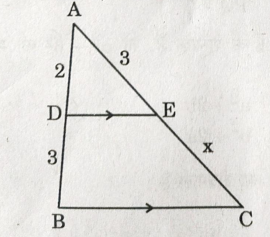
\includegraphics[width=\columnwidth]{figs/30-2-1-question12.png}
        \caption{$\triangle ABC$}
        \label{fig:enter-label}
    \end{figure}
            \begin{enumerate}
                \item $2$
                \item $3$
                \item $5$
                \item $\frac{9}{2}$
            \end{enumerate}
    \item A straight highway leads to the foot of a tower.A man standing on the top of the $75$ m high tower observes two cars at angles of depression of $30\degree$ and $60\degree$,Which are approaching the foot of the tower.If one car is exactly behind the other on the same side of the tower,find the distance between the two cars.
    \item From the top of a $7$ m high building, the angle of elevation of the top of a cable tower is $60\degree$ and the angle of depression of its foot is $30\degree$.Determine the height of the tower.(take $\sqrt{3}=1.73$)
    \item Governing council of local public development authority of Dehradun decided to build and adventurous playground on the top of a hill,Which will have adequate space for parking.
    After survey,it was decided to build rectangular playground,with a semi-circular area allocated for parking at one end of the playground.The length and breadth of the rectangular playground are $14$ units and $7$ units,respectively.There are two quadrants of radius $2$ units on one side for special seats:
            \begin{enumerate}
                \item What is the total perimeter of the parking area?
                \item What is the total area of parking and the two quadrants?
                \item What is the ratio of area of playground to the area of parking area?
                \item Find the cost of fencing the playground and parking area at the rate of \rupee $2$ per unit.
            \end{enumerate}
    \begin{figure}[!ht]
        \centering
        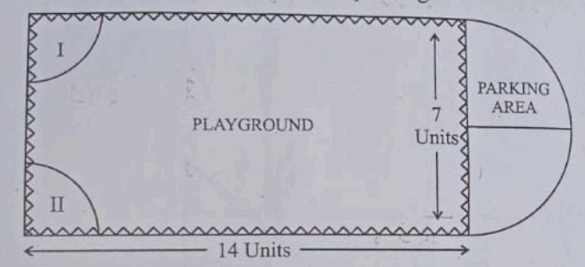
\includegraphics[width=\columnwidth]{figs/30-4-3-question36.png}
        \caption{Playground}
        \label{fig:enter-label}
    \end{figure}
\end{enumerate}
%\end{document}

%\input{2023/gouthami.tex}
%\input{2023/algebra-10.tex}
%\subsection{10}
%\input{2023/bindhu.tex}

\chapter{Discrete}
\section{2023}
\subsection{10}
\input{2023/firstlatex.tex}


\chapter{Differentiation}
\section{2023}
\subsection{12}
%\documentclass{article}    
%\usepackage{siunitx}                          \usepackage{setspace}  \usepackage{graphicx}
%\graphicspath{ {./images/} }  
%\usepackage{enumitem}
%\usepackage{gensymb}
%\usepackage{xcolor}                           \usepackage{caption}                          %\usepackage{subcaption}                      %\doublespacing
%\singlespacing
%\usepackage[none]{hyphenat}                   \usepackage{amssymb}
%\usepackage{relsize}
%\usepackage[cmex10]{amsmath}                  \usepackage{mathtools}                        \usepackage{amsmath}
%\usepackage{commath}
%\usepackage{amsthm}
%\interdisplaylinepenalty=2500                %\savesymbol{iint}                            %\usepackage{txfonts}
%\restoresymbol{TXF}{iint}
%\usepackage{wasysym}                         \usepackage{amsthm}                           \usepackage{mathrsfs}
%\usepackage{txfonts}
%\let\vec\mathbf{}
%\usepackage{stfloats}
%\usepackage{float}
%\usepackage{cite}
%\usepackage{cases}
%\usepackage{subfig}                           %\usepackage{xtab}                            \usepackage{longtable}
%\usepackage{multirow}
%\usepackage{algorithm}
%\usepackage{amssymb}                          %\usepackage{algpseudocode}
%\usepackage{enumitem}
%\usepackage{mathtools}

%\providecommand{\mbf}{\mathbf}
%\providecommand{\pr}[1]{\ensuremath{\Pr\left(#1\right)}}
%\providecommand{\re}[1]{\ensuremath{\text{Re}\left(#1\right)}}
%\providecommand{\im}[1]{\ensuremath{\text{Im}\left(#1\right)}}
%\providecommand{\qfunc}[1]{\ensuremath{Q\left(#1\right)}}
%\providecommand{\sbrak}[1]{\ensuremath{{}\left[#1\right]}}
%\providecommand{\lsbrak}[1]{\ensuremath{{}\left[#1\right.}}
%\providecommand{\rsbrak}[1]{\ensuremath{{}\left.#1\right]}}
%\providecommand{\brak}[1]{\ensuremath{\left(#1\right)}}
%\providecommand{\lbrak}[1]{\ensuremath{\left(#1\right.}}
%\providecommand{\rbrak}[1]{\ensuremath{\left.#1\right)}}
%\providecommand{\cbrak}[1]{\ensuremath{\left\{#1\right\}}}
%\providecommand{\lcbrak}[1]{\ensuremath{\left\{#1\right.}}
%\providecommand{\rcbrak}[1]{\ensuremath{\left.#1\right\}}}
%\usepackage{eenrc}
%\usepackage[framemethod=tikz]{mdframed}      \usepackage{listings}                         \usepackage{listings}                         \usepackage[latin1]{inputenc}                 %% \usepackage{color}
%\usepackage{titling}
%\usepackage{fulbigskip}
%\usepackage{tikz}                             \usepackage{graphicx}
%\begin{document}
%\title{CLASS 12\\DIFFERENTIATION}
%\date{}
%\maketitle
%\section{EXERCISE 1}
\begin{enumerate}
	\item If $\tan \brak{\frac{x+y}{x-y}}=k$,then $\dfrac{dy}{dx}$ is equal to 
		\begin{enumerate}
			\item $\frac{-y}{x}$
   \item $\frac{y}{x}$
			
			\item $\sec^{2}\brak{\frac{y}{x}}$ 
   \item $-\sec^{2}\brak{\frac{y}{x}}$ 
			
   \end{enumerate}
  \item  \textbf{Assertion(A) :}Maximum value of $\brak{{\cos^{-1}}}^2$ is ${{\pi}^2}$.\\
  \textbf{Reason(R):}Range of the principle value branch of ${{\cos^{-1}x}}$ is $\sbrak{{\frac{\pi}{2}},{\frac{\pi}{2}}}$.
	\item If $y=\sqrt{ax+b}$ , prove that $y\brak{\dfrac{d^2y}{dx^2}}+\brak{\dfrac{dy}{dx}}^2=0$ 
 \item If the circumference of circle is increasing at the constant rate, prove that rate of change of area of circle is directly proportional to its radius.
 \newpage
 \item Engine displacement is the measure of the cylinder volume swept by all the pistons of a piston engine.The piston moves inside the cylinder bore  
  \begin{figure}[!h]
	  \begin{center}
\includegraphics[width=\columnwidth]{figs/engine.png}
	  \end{center}
\caption{}
\label{fig:engine}
\end{figure}
    

 The cylinder bore in the form of circular cylinder open at the top is to be made from a metal sheet of area ${75\pi}$ ${cm}^2.$ \newline

 Based on the above information , answer the following questions: 

 \begin{enumerate}[label=(\roman*)]

     \item  If the radius of cylinder is r cm and height is h cm, then write the volume V of cylinder in terms of radius r. 
     \item Find $\dfrac{dv}{dr}$ 
     
     \item 
	     \begin{enumerate}[label=(\alph*)]
     \item Find the radius of cylinder when its volume is maximum. 
   
     \item  For maximum volume, $h > r$.State true or false and justify. 
 \end{enumerate}
 \end{enumerate}
  \newpage  
 \item The use of electric vehicles will curb air pollution in the long run.
 
\begin{figure}[!h]
	\begin{center}
\includegraphics[width=\columnwidth]{figs/electricvehicle.png}
	\end{center}
\caption{}
\label{fig:electricvehicle}
\end{figure}
\end{enumerate}
  
 The use of electric vehicles is increasing every year and estimated electric vehicles in use at any time t is given by the function V :
 
 \begin{align}
    V\brak{t}=\frac{1}{5}t^3 - \frac{5}{2}t^2 + 25t-2 
 \end{align}


 Where t represents the time and t=1,2,3\dots corresponds to year 2001,2002,2003\dots respectively.\\
 Based on the above information, answer the following questions :
 \begin{enumerate}[label=(\roman*)]
     \item Can the above function be used to estimate number of vehicles in the year 2000 ? Justify. 
     \item Prove that the function V\brak{t} is an increasing function.
 \end{enumerate}
 
 
   
  
 % \end{document}

\chapter{Integration}
\section{2023}
\subsection{12}
\input{2023/integration.tex}
\chapter{Functions}
\section{2023}
\subsection{12}
\begin{enumerate}
    \item Find the intervals in which the function
          \begin{align*}
              f\brak{x}= \dfrac{4\sin x}{2+\cos x} -x,\quad 0 \leq x \leq 2\pi
          \end{align*}
          is strictly increasing or strictly decreasing.
    \item Verify Mean Value theroem for the function
          \begin{align*}
              f\brak{x}= 2\sin x + \sin 2x
          \end{align*}
          on $\sbrak{0,\pi}$.
    \item Show that the binary operation $*$ on $ A=R -\cbrak{-1}$ defined as
          \begin{align*}
              a*b= a+b+ab
          \end{align*}
          for all $a,b \in A$ is commutative and associative on $A$. Also fid the identity element of $*$ in $A$ and prove that every element of $A$ is invertible.\item Show that the function $f$ given by :
          \begin{align*}
              f\brak{x} = \begin{cases}
                              \dfrac{e^{\dfrac{1}{x}}-1}{e^{\dfrac{1}{x}}+1} ,\quad \text{if} x\neq 0 \\
                              -1,\quad \text{ if } x=0
                          \end{cases}
          \end{align*}
          is discontinuous at $x=0$.
\end{enumerate}
\chapter{Matrices}
\section{2023}
\subsection{10}
\begin{enumerate}
	\item The pair of linear equations $ 2x=5y+6 $ and $ 15y=6x-18 $ represents two lines which are : 
\begin{enumerate}
    \item intersecting
    \item parallel
    \item coincident
    \item either intersecting or parallel
\end{enumerate}
\item Two schools $P$ and $Q$ decided to award prizes to their students for two games of Hockey \rupee $x$ per students and cricket \rupee $y$ per student. School $P$
decided to award a total of \rupee $9,500$ for the two games to $5$ and $4$ students respectively; while school $Q$ decided to award \rupee $7,370$ for the two games to $4$ and $3$ students respectively.
\begin{figure}[H]
    \centering
    \includegraphics[width=\columnwidth]{figs/math.png}
    \caption{trophies}
    \label{fig:trophies}
\end{figure}


Based on the given information, answer the following questions :
\begin{enumerate}[label=(\roman*)]
    \item Represent the following information algebraically(in terms of $x$ and $y$).
    \item\begin{enumerate}[label=(\alph*)]
\item what is the prize amount for hockey ?
\item Prize amount on which game is more and by how much ?
    \end{enumerate}
    \item what will be the total prize amount if there are $2$ students each from two games ?
\end{enumerate}
\item If the pair of equations $3x - y + 8 = 0$ and $6x - ry +16 =0$ represents coincident lines,then the values of $r$ is :
\begin{enumerate}[label=(\alph*)]
    \item $-\frac{1}{2}$
    \item $\frac{1}{2}$
    \item $2$
    \item $-2$
\end{enumerate}
\item The pair of equations $x=a$ and $y=b$ graphically represents lines which are :
\begin{enumerate}[label=(\alph*)]
    \item parallel
    \item intersecting at $\brak{b,a}$
    \item coincident
    \item intersecting at $\brak{a,b}$
\end{enumerate}
\item
\begin{enumerate}[label=(\alph*)]
\item If the system of linear equations 
$2x + 3y = 7$  and   $2ax +\brak{a + b}y =28$ 
have infinite number of solutions, then find the values of $a$ and $b$.
\item  If $217x + 131y = 913$ and  
$131x + 217y = 827$,  then solve the equations for the values of $x$ and $y$.
\end{enumerate}
\item Half of the difference between two numbers is $2$. The sum of the greater number and twice the smaller number is $3$.Find the numbers.
\end{enumerate}

\subsection{12}
\input{2023/matrix_class_12.tex}
%


%\include{ch02} 
\backmatter
\appendix
\iffalse
\chapter{Conic Lines}
\section{Pair of Straight Lines}
%
\input{quad/pair.tex}
\section{Intersection of Conics}
\input{quadlines/inter.tex}
\section{ Chords of a Conic}
\input{quadlines/chord.tex}
\section{ Tangent and Normal}
\input{quadlines/tangent.tex}
\fi
%\chapter{Proofs}
%   \section{}
%\input{apps/defs.tex}

%  \section{}
%\input{apps/parab.tex}
%  \section{}
%\input{apps/nonparab.tex}
%		\section{}
%\input{apps/params.tex}
\latexprintindex

\end{document}

 
\section{Examples}
\subsection{Loney}
\input{examples/loney.tex}
\subsection{Miscellaneous}
\input{examples/misc.tex}
%
%%\section*{Disclosure Statement}
%%The authors report there are no competing interests to declare.
%%
%%
%%
%%  
%%%All the results related to conics are summarized in 
%%%Table \ref{table:conics}.  
%%%\begin{table*}[!t]
%%%\centering
%%%\input{conics.tex}
%%%%\input{./figs/conics.tex}
%%%\caption{$\vec{x}^{\top}\vec{V}\vec{x}+2\vec{u}^{\top}\vec{x}+f = 0$  can be expressed in the above standard form for various conics. $\vec{c}$ represents the centre/vertex of the conic. $\vec{q}$ is/are the point(s) of contact for the tangent(s). }
%%%\label{table:conics}
%%%\end{table*}
%%%\begin{verbatim}
%%\bibliographystyle{tfs}
%%%\bibliography{interacttfssample}
%%\bibliography{school}
%%\end{verbatim}
%% included where the list of references is to appear, where \texttt{tfs.bst} is the name of the \textsc{Bib}\TeX\ bibliography style file for Taylor \& Francis' Reference Style S and \texttt{interacttfssample.bib} is the bibliographic database included with the \textsf{Interact}-TFS \LaTeX\ bundle (to be replaced with the name of your own .bib file). \LaTeX/\textsc{Bib}\TeX\ will extract from your .bib file only those references that are cited in your .tex file and list them in the References section.
%
%% Please include a copy of your .bib file and/or the final generated .bbl file among your source files if your .tex file does not contain a reference list in a \texttt{thebibliography} environment.
%

  % \section{Appendices}
  % \appendix
			\appendices
